\documentclass[a4paper,12pt]{article}
\usepackage[utf8x]{inputenc}
\usepackage[pdftex]{color,graphicx}
\usepackage[hypertexnames=false]{hyperref}
\usepackage[german,ngerman]{babel}
\usepackage{fancyhdr}
\usepackage{amssymb}
\usepackage[pages=some]{background} % Draft Wasserzeichen mit Option pages=all sonst pages=some
\usepackage{amsmath}
\usepackage{svg}
\usepackage[rflt]{floatflt}
\usepackage{tabularx}
\usepackage{ausarbeitung}
\usepackage{bookmark}
\usepackage{cite}
\usepackage{graphicx}
\usepackage{caption}
\usepackage{subcaption}
\usepackage{listings}

%% Diese Farben werden f�r den Quelltext verwendet
\definecolor{srcblue}{rgb}{0,0,0.5}
\definecolor{srcgray}{rgb}{0.5,0.5,0.5}
\definecolor{srcred}{rgb}{0.5,0,0}
%% Diese Zeile unbedingt stehen lassen und anpassen - sie enthält Autor und Titel der Ausarbeitung
\mywork{Lars Hick}{Lastverteilung von HTTP/2-Anfragen in Kubernetes}

\begin{document}
    %% Bei Diplomarbeiten folgende Zeile nutzen
    %%\mydiplomtitle{(ggf. Name des Betreuers)}
    %% Bei Bachelorarbeiten diese Zeile auskommentieren
    %%\mybachelortitle{(ggf. Name des Betreuers)}
    %% Bei Seminararbeiten diese Zeile auskommentieren
    \myseminartitle{Moderne Programmiertechniken und -Methoden}{Daniela Keller}

    %% Inhaltsverzeichnis
    %% frontmatter setzt die Seitenzahlen auf i, ii, ...
    \frontmatter

    %% Generiert automatisch aus den Sektionsbefehlen ein Inhaltsverzeichnis
    \tableofcontents

    \newpage

    \section*{Überblick}
    Kubernetes ist im Cloud Nativen Bereich zu einem Industriestandard zur Container Orchestrierung geworden.
    In Kombination mit dem HTTP/2 Protokoll bietet Kubernetes jedoch immer noch einige Fallstricke, die es bei der Entwicklung und Bereitstellung einer auf beiden Technologien basierenden Anwendung zu beachten gibt.
    Zu Begin werden in Kapitel~\ref{sec:grundlagen} die verwendeten Technologien sowie deren Grundlagen dargestellt.
    Nachdem der Grundstein gelegt ist, wird in Kapitel~\ref{sec:kernkapitel} eine Beispielanwendung vorgestellt, welche als Referenz HTTP/1 verwendet und an der anschließend verschiedene Möglichkeiten zur Lastverteilung von HTTP/2 Anfragen in einem Kubernetes Cluster exerziert werden.
    Diese Implementierungen liefern genug Metriken, um sie miteinander zu vergleichen.
    Der Vergleich zwischen den Implementierungen mit Blick auf quantitativ messbare wie Fairness, Performance und qualitative wie die Nutzbarkeit wird in Kapitel~\ref{sec:auswertung} getroffen.
    Abschließend wird in Kapitel~\ref{sec:fazit} das Ergebnis der Arbeit bewertet sowie in Kapitel~\ref{sec:ausblick} Grundlage für weitere Forschung gegeben.
    \newpage

    %% das Mainmatter sorgt für die Nutzung arabischer Seitenzahlen
    \mainmatter

    \section{Grundlagen}\label{sec:grundlagen}
    Dieses Kapitel gibt einen Überblick über verwendete Technologien und Konzepte.
Zunächst werden relevante Protokolle und deren Funktionsweise erläutert.
Anschließend wird eine Einführung über Kubernetes gegeben.

\subsection{Hypertext Transfer Protocol}\label{subsec:hyper-text-transfer-protocol}

Das Hypertext Transfer Protocol (HTTP) ist ein Protokoll zur Kommunikation über das World Wide Web, welches von der Internetengineering Task Force (IETF) standardisiert und weiterentwickelt wird.
Da HTTP sich im OSI-Modell der Anwendungsschicht zuordnen lässt, bringt das Protokoll unter anderem die Vorteile mit sich, dass es unabhängig von der darunterliegenden Netzwerktechnologie und einfach erweiterbar ist.
So bildet HTTP die Grundlage für viele weitere Protokolle wie zum Beispiel Hypertext Transfer Protocol Secure (HTTPS)~\cite{rfc2818} zur verschlüsselten Übertragung von Daten oder das Simple Object Access Protocol (SOAP)~\cite{SOAP-20000508} zur Kommunikation zwischen verteilten Systemen.
Aufgrund seiner Erweiterbarkeit und einiger Performance Optimierungen in der Vergangenheit liegt HTTP heute in den Versionen 1.0, 1.1 und 2 vor.
Eine version 3 ist momentan in Entwicklung.
Die folgenden Abschnitte gehen kurz auf für die folgende Arbeit relevante versionsspezifische Besonderheiten ein.

\subsubsection{HTTP/1.0 und HTTP/1.1}
HTTP ist ein textbasiertes, zustandsloses Protokoll, was bedeutet, dass sogenannte aus Klartext bestehende Anfragen (Requests) unabhängig voneinander sind.
Dieser Umstand erlaubt die horizontale Skalierung von Webservern und vereinfacht deren Implementierung.
RFC1945~\cite{rfc1945} spezifiziert HTTP/1.0.
Zur Spezifikation gehört die Definition von Unique Resource Identifiers (URIs), welche gemeinhin bekannt sind als Internetadresse.
Des Weiteren erfolgt die Definition verschiedener HTTP-Methoden wie unter anderen \textit{GET} (Informationsabfrage), \textit{HEAD} (Metadatenabfrage) und \textit{POST} (Hochladen von Informationen) und Status Codes zur Auswertung der Server Antwort (Response).
Nach HTTP/1.0 wird für jeden Request eine neue TCP-Verbindung etabliert, welche nach Übertragung der Antwort wieder geschlossen wird.

Da mit HTTP/1.0 die Grundlagen zur Kommunikation im Web gelegt sind, wird das Protokoll in RFC2616~\cite{rfc2616} um Version HTTP/1.1 erweitert.
Im Wesentlichen werden mit der neuen Version die folgenden Punkte zur Verbesserung der Performance eingeführt:

\begin{itemize}
    \item \textbf{Persistente Verbindungen:} TCP Verbindungen, welche zwischen Client und Server aufgebaut werden, werden wiederverwendet, anstatt geschlossen zu werden.
    Diese Konfiguration wird in HTTP/1.1 zum Standard, reduziert den Overhead des TCP-Handlings und führt zu schnelleren Antwortzeiten.
    \item \textbf{Pipelining:} Persistente Verbindungen erlauben das Senden mehrerer paralleler Requests, ohne auf die Antwort des Servers zu warten.
    \item \textbf{Chunked Transfer-Encoding:} Daten können in mehreren Teilen übertragen werden.
    Dieses Verhalten erlaubt das Streaming von Daten.
\end{itemize}

\subsubsection{HTTP/2}

Obwohl HTTP/1.1 mit dem Pipelining bereits die parallele Übertragung von Requests ermöglicht, birgt diese Technologie einige Nachteile.
So können beim Pipelining über persistente Verbindungen zu unterschiedlichen Anwendungsszenarien Head of Line Blocking Probleme auftreten.
Obwohl die Anfragen parallel und ohne auf die Antwort zu warten abgeschickt werden, müssen die Antworten in der entsprechenden Reihenfolge vom Server zurückgegeben werden.
Im schlimmsten Fall geht eine Antwort verloren und die komplette Warteschlange muss auf die erneute Sendung der Antwort warten.
Schnellere Requests werden so durch langsamere blockiert und schlussendlich erfolgt trotzdem eine sequentielle Abarbeitung der Anfragen~\cite{7179400}.

HTTP/2 bringt mit dem Multiplexing eine Neuerung, welche die Problematik des Head of Line Blocking reduziert.
Da die Request-/Response-Paare nun unabhängig voneinander über eine Verbindung multiplexed werden können, ist die Reihenfolge der empfangenen Antworten nun irrelevant.
Wichtig zu erwähnen ist, dass Multiplexing das Head of Line Blocking Problem auf HTTP-Ebene eliminiert, jedoch nicht auf TCP-Ebene.
Neben Multiplexing und weiteren Neuerungen bringt HTTP/2 außerdem die Priorisierung von Requests, wie auch binäre Kodierung und Kompression von Header Feldern mit sich, was zu wesentlich kleineren Paketgrößen und damit schnelleren Übertragungsraten führt.
HTTP/2 ist abwärtskompatibel zu seinen Vorgängern und wird in RFC9113~\cite{rfc9113} spezifiziert.

Corbel et al. zeigen in ihrer Arbeit \textit{HTTP/1.1 pipelining vs HTTP2 in-the-clear: Performance comparison}~\cite{7745823} die Performanceverbesserungen von HTTP/2 gegenüber HTTP/1.1 auf.

\subsection{gRPC}\label{subsec:grpc}
gRPC ist ein von Google entwickeltes, auf HTTP/2 basierendes Remote Procedure Call (RPC) Framework, welches Quelloffen zur Verfügung gestellt wird.
Das Framework bringt die Besonderheit mit, dass Schnittstellendefinitionen Programmiersprachenunabhängig in der Interface Definition Language (IDL) namens Protocol Buffers Language (protobuf)~\cite{protobuf} definiert werden können.
Die Abstraktion der Schnittstellendefinitionen von der Implementierung erlaubt die Entwicklerübergreifende Verständigung auf eine gemeinsame Schnittstelle.
Zudem bietet das Framework einen Compiler an, welcher die Schnittstellendefinitionen sowohl in Server-, als auch in Client-Code in einer Vielzahl von Programmiersprachen übersetzen kann.
Mit gRPC kann ein strikter API-First Ansatz verfolgt werden, welcher die Entwicklung von Client und Server unabhängig voneinander ermöglicht.
Da gRPC auf HTTP/2 basiert, welches von der kompletten Infrastruktur auf dem Weg zwischen Client und Server unterstützt sein muss, bietet sich gRPC vor allem zur Kommunikation zwischen verschiedenen Komponenten innerhalb eines Kubernetes Clusters an, wo die komplette Kommunikationsstrecke technisch in einer Hand liegen.

\subsection{Kubernetes}\label{subsec:kubernetes}
Das Kapitel im Anschluss führt in das Software Ökosystem Kubernetes ein.
Zu Beginn wird ein grundlegender Überblick über die Architektur und die Funktionsweise gegeben.
Danach werden einige in der Praxis oft verwendete Komponenten und deren Konzepte erläutert.
Da Kubernetes ein sehr umfangreiches Ökosystem ist, wird in diesem Kapitel ausschließlich auf die für die Arbeit relevanten und daher sich in Nutzung befindlichen Komponenten eingegangen.

\subsubsection{Kubernetes Control Plane}

Kubernetes ist ein von Google entwickeltes Container Orchestration Framework.
Für die Cloud-Native Entwicklung eignet es sich besonders gut als Abstraktion mehrerer virtueller Maschinen für eine einfachere, hardware unabhängige Bereitstellung von Anwendungen, welche hoch verfügbar oder skalierbar sein sollen.
Ein wesentlicher Bestandteil von Kubernetes ist die Control Plane, welche die zentrale Steuerung des Clusters zur Aufgabe hat.
Die Control Plane besteht aus mehreren Komponenten, welche je nach Anwendungsfall in einer High-Availability Konfiguration laufen können.
In jedem Fall besteht die Control Plane aus folgenden Komponenten:
\begin{itemize}
    \item \textbf{API Server:} Über den API Server erfolgt die Kommunikation mit Kubernetes und der Control Plane.
    Jede Interaktion mit einer Kubernetes Ressource lässt sich auf einen zugrunde liegenden Schnittstellen Aufruf an den API Server zurückführen.
    \item \textbf{Controller Manager:} Eine Sammlung verschiedenster Kontrollprozesse, welche nach dem Unix Principle \emph{Do One Thing and Do It Well}~\cite{gancarz2003linux} aufgeteilt sind.
    \item \textbf{etcd:} Ein Key-Value-Store, welcher als Persistenz für das Cluster und dessen State dient.
    \item \textbf{Scheduler:} Der Scheduler übernimmt die Aufgabe, Pods auf freie Nodes zu verteilen.
\end{itemize}

Des Weiteren befinden sich in einem Kubernetes Cluster, bestehend aus mehreren Virtual Machines (VMs), welche in diesem Kontext auch als Node bezeichnet werden, auf jedem Node folgende Komponenten:

\begin{itemize}
    \item \textbf{Kubelet:} Das Kubelet stellt sicher, dass provisionierte Pods entsprechend ihrer Konfiguration laufen.
    \item \textbf{kube-proxy:} Stellt die Kommunikation der Kubernetes Komponenten miteinander sicher.
\end{itemize}
Die Linux Foundation bietet eine ausgezeichnete Dokumentation zur weitgehenderen Lektüre in die Kubernetes Control Plane~\cite{kubernetescomponents}.
\subsubsubsection{Pod}
Der Pod ist die kleinste kubernetesspezifische Einheit.
Er besteht aus einem oder mehreren Containern, welche konform der Standards der Open Container Initiative sind.
Die unter Entwicklern am weitesten verbreitete Methode, Container zu bauen, ist mit Hilfe von Docker.
Der Pod fungiert als ein Wrapper um seine Container, um diese als eine Einheit zu behandeln und in das Kubernetes Ökosystem integrierbar zu machen.
Die Hauptaufgabe des Pods ist es, Informationen über Ressourcenverbrauch sowie den Gesundheitszustand des Stücks Software, welches in den Containern läuft, zu sammeln und der Control Plane bereitzustellen.
Wird ein Pod aktualisiert, so muss dieser neu gestartet werden, da es sich dabei um eine unveränderliche Einheit handelt.

\subsubsubsection{Deployment}
Mehrere Pods, welche die Konfiguration und bereitgestellten Container teilen, können in einem Deployment zusammengefasst werden.
Ein Deployment bietet die Möglichkeit, mehrere Pods des gleichen Typs zentral zu verwalten.
So wird durch diese Komponente eine Vielzahl für moderne Softwaretechnik relevanter Funktionen bereitgestellt:

\begin{itemize}
    \item \textbf{Skalierbarkeit:} Die Anzahl der gleichzeitig laufenden Pods kann über ein Deployment definiert werden.
    So können High availability Anforderungen durch einfache Konfiguration des Deployments erfüllt werden.
    \item \textbf{Rolling Updates:} Liegt Software in einer neuen Version vor, so muss diese auch ausgerollt werden.
    Wie oben geschrieben, kann der Container in einem Pod nicht einfach ausgetauscht werden.
    Durch rolling Updates wird sichergestellt, dass die neue Softwareversion in neuen Pods bereitsteht, bevor Pods mit der alten Version heruntergefahren werden.
    \item \textbf{Rollbacks:} Wurde eine Version bereitgestellt, welche fehlerhaft ist, so kann über ein Deployment einfach die vorherige Version wiederhergestellt werden.
\end{itemize}

\subsubsubsection{Service}
Um ein Deployment verfügbar zu machen, kann ein Service definiert werden.
Je nach Typ erfüllt ein Service unterschiedliche Funktionen.
Laut Dokumentation~\cite{kubernetesservices}existieren die folgenden:

\begin{itemize}
    \item \textbf{ClusterIP:} Der Service erhält eine IP-Adresse, welche nur innerhalb des Clusters erreichbar ist.
    \item \textbf{NodePort:} Erlaubt den externen Zugriff auf den Service über das entsprechende Protokoll und den Port.
    Ermöglicht zudem die eigene Implementierung eines Loadbalancing verfahrens.
    \item \textbf{LoadBalancer:} Ist das Kubernetes Cluster über einen Cloud-Provider provisioniert, so wird in diesem Fall automatisch ein Loadbalancer für den Service erstellt, welcher auf diesen verweist.
    \item \textbf{ExternalName:} Erlaubt das direkte Mapping eines DNS Names auf einen Service.
\end{itemize}

\subsubsection{Custom Resource Definitions}
Jede Interaktion mit einem Kubernetes Cluster stellt einen API-Aufruf an die Control Plane dar.
Custom Resource Definitions ermöglichen es dem Verwalter eines Kubernetes Cluster, diese API um eigene Ressourcen zu erweitern, welche dann über die typischen Kubernetes Definitionen bereitgestellt werden.

\newpage


    \section{Kernkapitel}\label{sec:kernkapitel}
    Folgendes Kapitel erläutert den Aufbau der Testanwendung.
Zu Beginn wird die Anwendung für einen Verbindungsaufbau über HTTP/1 konfiguriert.
Anschließend wird die Problematik mit HTTP/2 in der Standardkonfiguration und verschiedene Lösungsansätze dafür dargestellt.
Da es sich beim HTTP/1 Load Balancing um den normalen Anwendungsfall für Kubernetes Loadbalancing handelt, dient dies zur Referenz in den anschließenden Konfigurationen, welche die Anwendung im gRPC-Modus und somit über HTTP/2 ausführen.
Der gesamte Code der Anwendung ist online einsehbar \cite{github}.

\subsection{Anwendungsaufbau}\label{subsec:anwendungsaufbau}
Das Kapitel gibt einen Überblick über den generellen Aufbau der Anwendung, um evaluierbare Daten zu generieren.
Des Weiteren wird ein Überblick gegeben, wie generierte Daten von der implementierten Anwendung abgerufen und visuell dargestellt werden können.

\subsubsection{Client-Server-Architektur}
Da nicht die Anwendung selbst, sondern die Kommunikation zwischen zwei unterschiedlichen Pods und deren Replicas im Vordergrund steht, wird eine einfache Client-Server-Anwendung entwickelt.

Der Server stellt hierbei eine Schnittstelle zur Verfügung.
Um einen gewissen Rechenaufwand zu erzeugen, berechnet die aufrufbare Schnittstelle für einen gegebenen Wert über das Heron Verfahren die Wurzel und gibt das Ergebnis als Antwort an den Aufrufer zurück.

Dem Server gegenüber steht der Client, welcher in regelmäßigen, konfigurierbaren Zeit\-ab\-stän\-den eine randomisiert ausgewählte Zahl an die vom Server bereitgestellte Schnittstelle als Anfrage sendet und auf die Antwort mit dem Ergebnis vom Server wartet, bevor eine nächste Anfrage abgesetzt wird.

Über Command Line Argumente können beide Anwendungen in folgenden verschiedenen Modi gestartet werden, welche in den referenzierten Sektionen detaillierter vorgestellt werden:
\begin{itemize}
    \item HTTP/1~(\ref{subsec:http/1-load-balancing})
    \item HTTP/2 Standard~(\ref{subsubsec:standard})
    \item HTTP/2 headless Service~(\ref{subsubsec:headless})
    \item HTTP/2 Service Mesh~(\ref{subsubsec:mesh})
\end{itemize}
Für jeden Laufmodus wird die Anwendung in einem separaten Kubernetes Namespace vorkonfiguriert bereitgestellt.
Aus Gründen der Vorhersehbarkeit wird auf Horizontal Pod Autoscaler und somit auf die automatische Skalierung der Anwendung auf Basis von Ressourcenmetriken verzichtet.

\subsubsection{Auswertbarkeit}\label{subsubsec:auswertbarkeit}
Um auswertbare Daten zu erhalten, stellen sowohl Server- als auch Client eine weitere Schnittstelle bereit, welche frei definierbare Metriken exponiert und einem Scraper zur regelmäßigen Abfrage zur Verfügung stellt.
Grafik~\ref{fig:setup} visualisiert das komplette Setup, wobei die Client-Server-Anwendung, welche auf mehrere Namespaces in unterschiedlichen Konfigurationen läuft, abstrahiert dargestellt wird:

\begin{figure}[H]
    \centering
    \includesvg[width=0.8\linewidth]{img/architektur.svg}
    \caption{Anwendungsarchitektur}
    \label{fig:setup}
\end{figure}

Wie zu erkennen ist, wird zur Datenanalyse der Cloud Native Metrik-Scraper Prometheus und zur Darstellung der Daten das Tool Grafana verwendet.
Das zur Verfügung gestellte Repository kommt mit einem vorkonfigurierten Dashboard, welches für jeden Laufmodus die folgenden Metriken visualisiert:
\begin{itemize}
    \item Anzahl Pods pro Client und Server
    \item Requests pro Sekunde für jeden Server Pod
    \item Client Latenz im 99ten, 95ten Perzentil sowie Median
\end{itemize}

Um verschiedene Skalierungsszenarien zu simulieren, wird für jede Laufvariante der in Grafik~\ref{fig:zeitablauf} dargestellte zeitliche Ablauf festgelegt:

\begin{figure}[H]
    \centering
    \includesvg[width=0.5\linewidth]{img/zeitablauf.svg}
    \caption{Interaktionen mit dem Kubernetes Cluster}
    \label{fig:zeitablauf}
\end{figure}

Der Server startet mit zwei und der Client mit einer Instanz.
Da gRPC, wie in Sektion~\ref{subsec:grpc} erwähnt, vorwiegend zur In-Cluster Kommunikation verwendet werden sollte, besteht sowohl für den Server, als auch für den Client die Notwendigkeit, bei Bedarf variabel skalierbar zu sein.
Ersteres Szenario wird durch die Skalierung des Servers abgedeckt.
Bevor der Client skaliert und somit ein erhöhtes Anfrageaufkommen für den Server generiert wird, wird dieser neu gestartet.
Dies dient zur Veranschaulichung eines Sonderfalls, auf welchen in Absatz~\ref{subsubsec:headless} eingegangen wird.

\subsubsection{Weitere Tools und Hardware}
Zur Bereitstellung des Kubernetes Clusters wird auf das Tool ctlptl von tilt zurückgegriffen.
Dieses ist so konfiguriert, dass ein Kubernetes Cluster mit Hilfe von KinD (Kubernetes in Docker) provisioniert wird.
Das Cluster umfasst einen Knoten für die Control Plane sowie vier weitere Knoten als Worker.
Die im Folgenden vorgestellten Ergebnisse werden auf einem Macbook Pro mit einem Apple M2 Pro und 16 GB RAM ermittelt.

\newpage

\subsection{HTTP/1 Load Balancing}\label{subsec:http/1-load-balancing}
Zum Zeitpunkt der Entwicklung von Kubernetes handelte es sich bei HTTP/1 bereits um einen weit verbreiteten Industriestandard für das Web.
Daher basieren heute viele Webanwendungen sowie Webserver auf dem Protokoll, weswegen das Container Orchestration Framework Load Balancing über HTTP/1 standardmäßig unterstützt.
Um für das folgende Kapitel, welches sich mit HTTP/2 Load Balancing beschäftigt, Werte zu liefern, die repräsentieren, wie die Lastverteilung in einer funktionierenden Anwendung aussehen sollten, wird die vorgestellte Anwendung im HTTP/1 bzw. REST-Modus ausgeführt.
\begin{figure}[H]
    \centering
    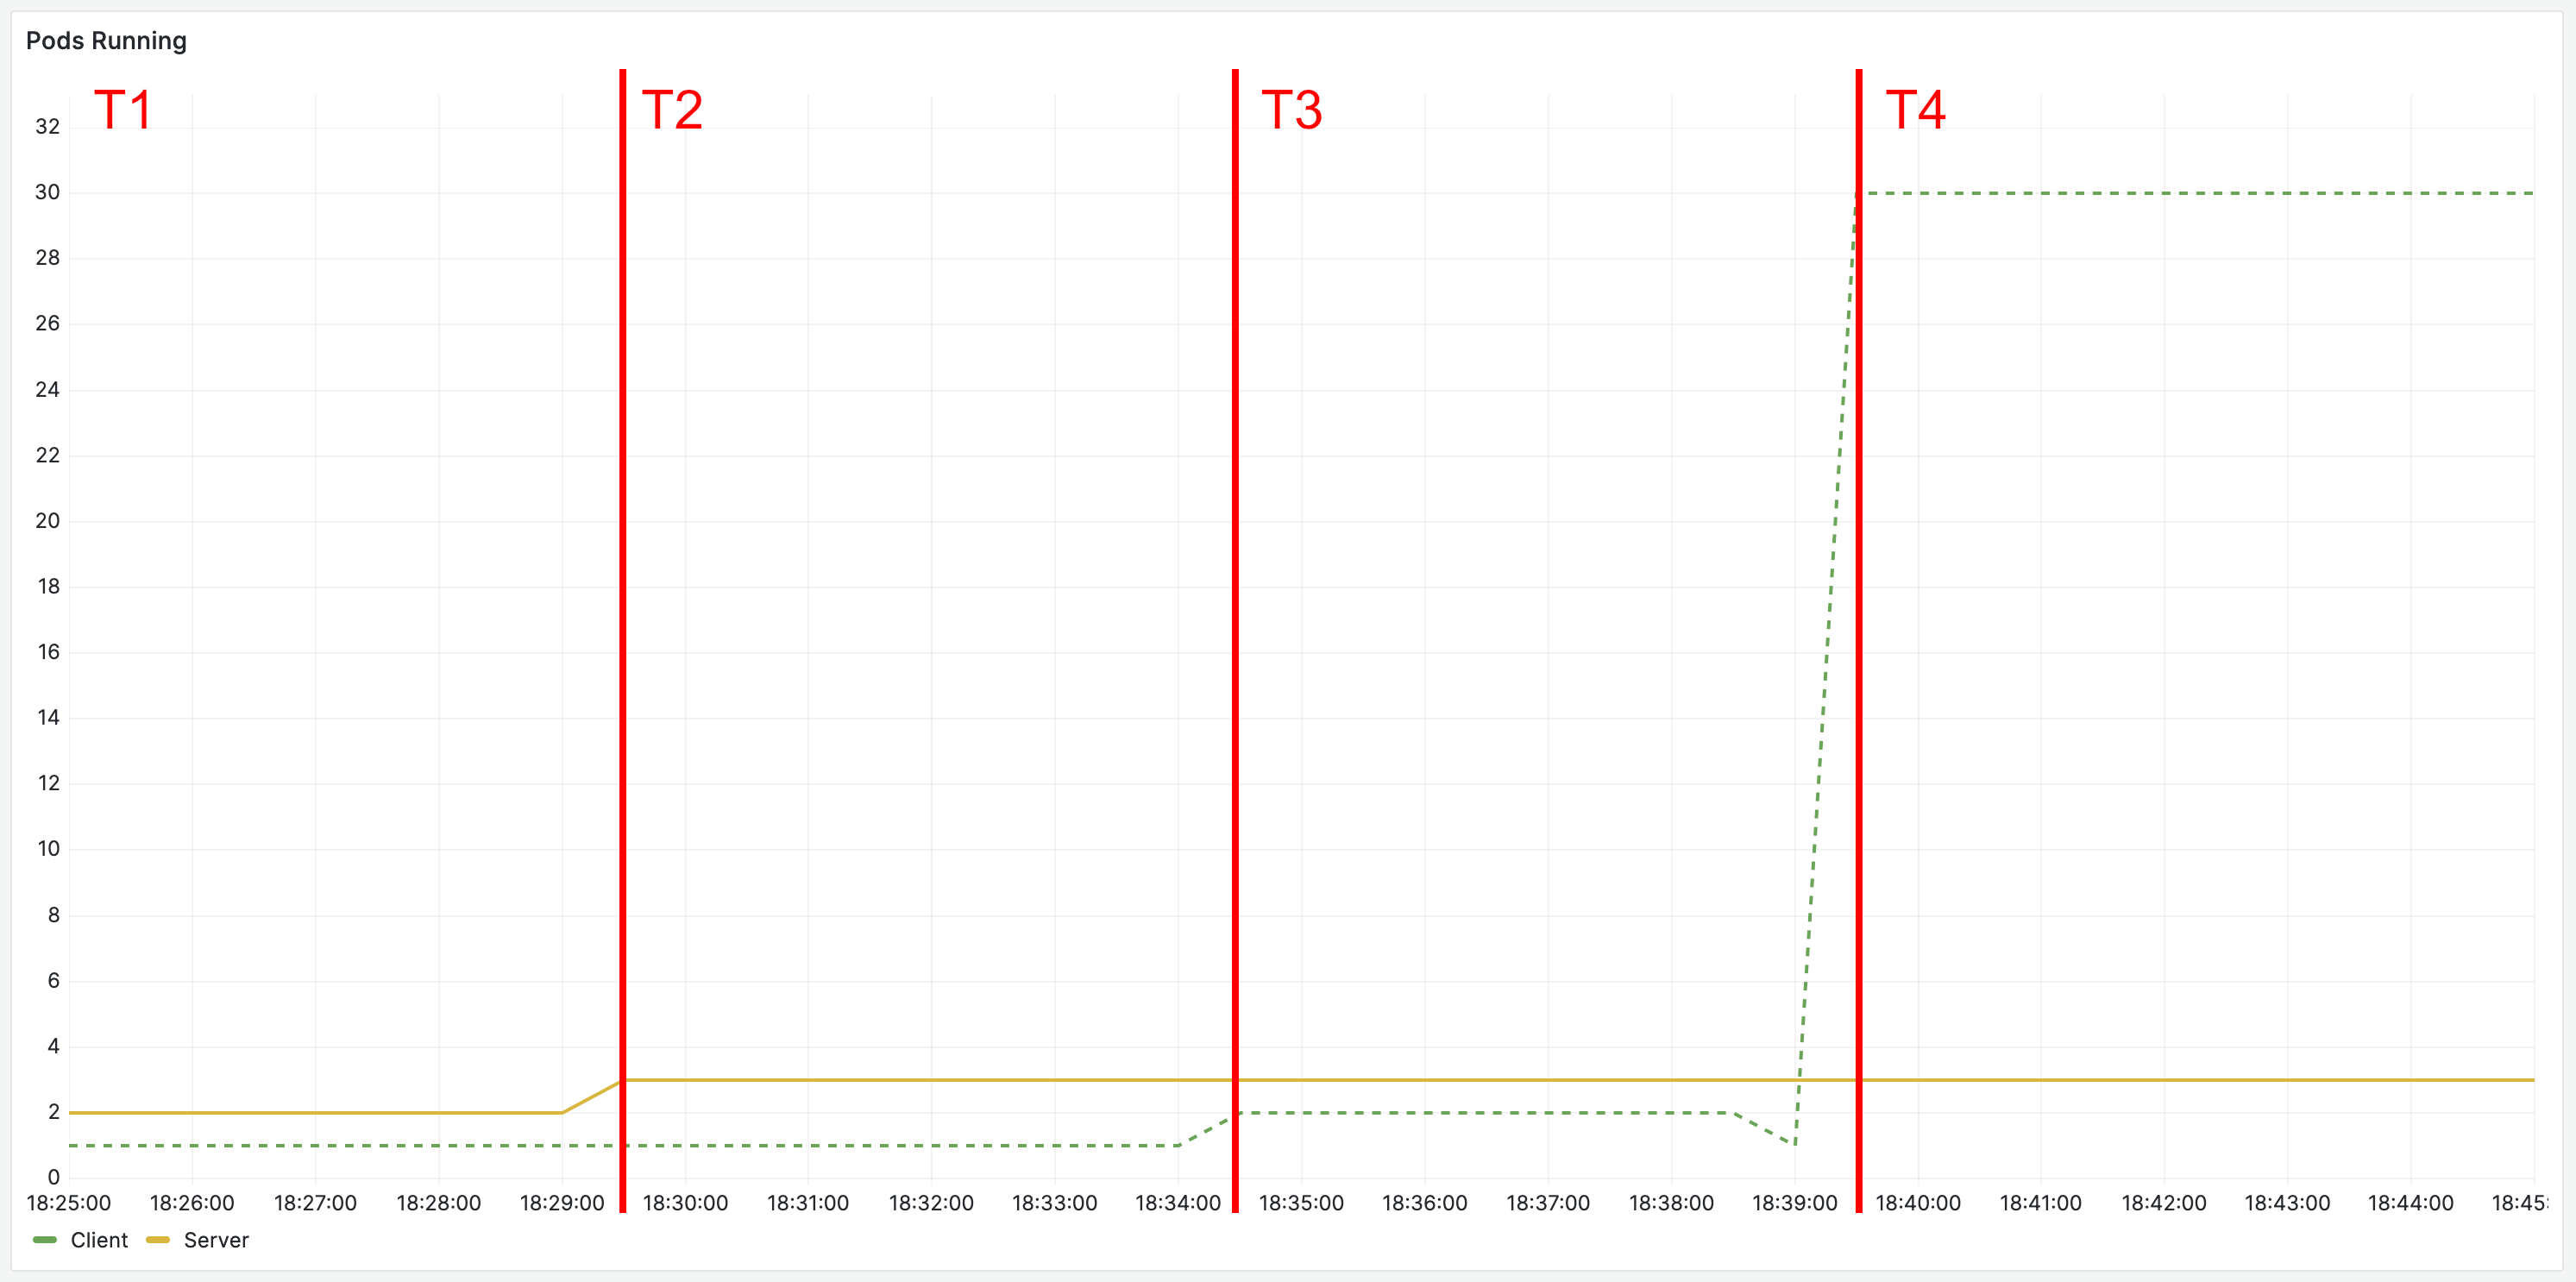
\includegraphics[width=0.75\textwidth]{img/rest_pods}
    \caption{Client (gestrichelt) und Server (durchgezogen) Pods}
    \label{fig:rest_pods}
\end{figure}

Grafik~\ref{fig:rest_pods} visualisiert den Verlauf der Replicagröße beider Deployments.
Die folgenden Zeitpunkte sind hierbei besonders von Relevanz:
\begin{itemize}
    \item \textbf{T1}: Server startet mit zwei Instanzen, der Client mit einer.
    \item \textbf{T2}: Der Server wird auf drei Instanzen skaliert
    \item \textbf{T3}: Der Client wird neu gestartet.
    \item \textbf{T4}: Der Client wird auf dreißig Instanzen skaliert.
\end{itemize}

Da von diesem Verhalten in den Absätzen~\ref{subsubsec:standard},~\ref{subsubsec:headless} und~\ref{subsubsec:mesh} nicht abgewichen wird und die Zeitpunkte als Referenz nun erläutert wurden, wird auf eine erneute Darstellung dessen im Folgenden verzichtet.

\begin{figure}[H]
    \centering
    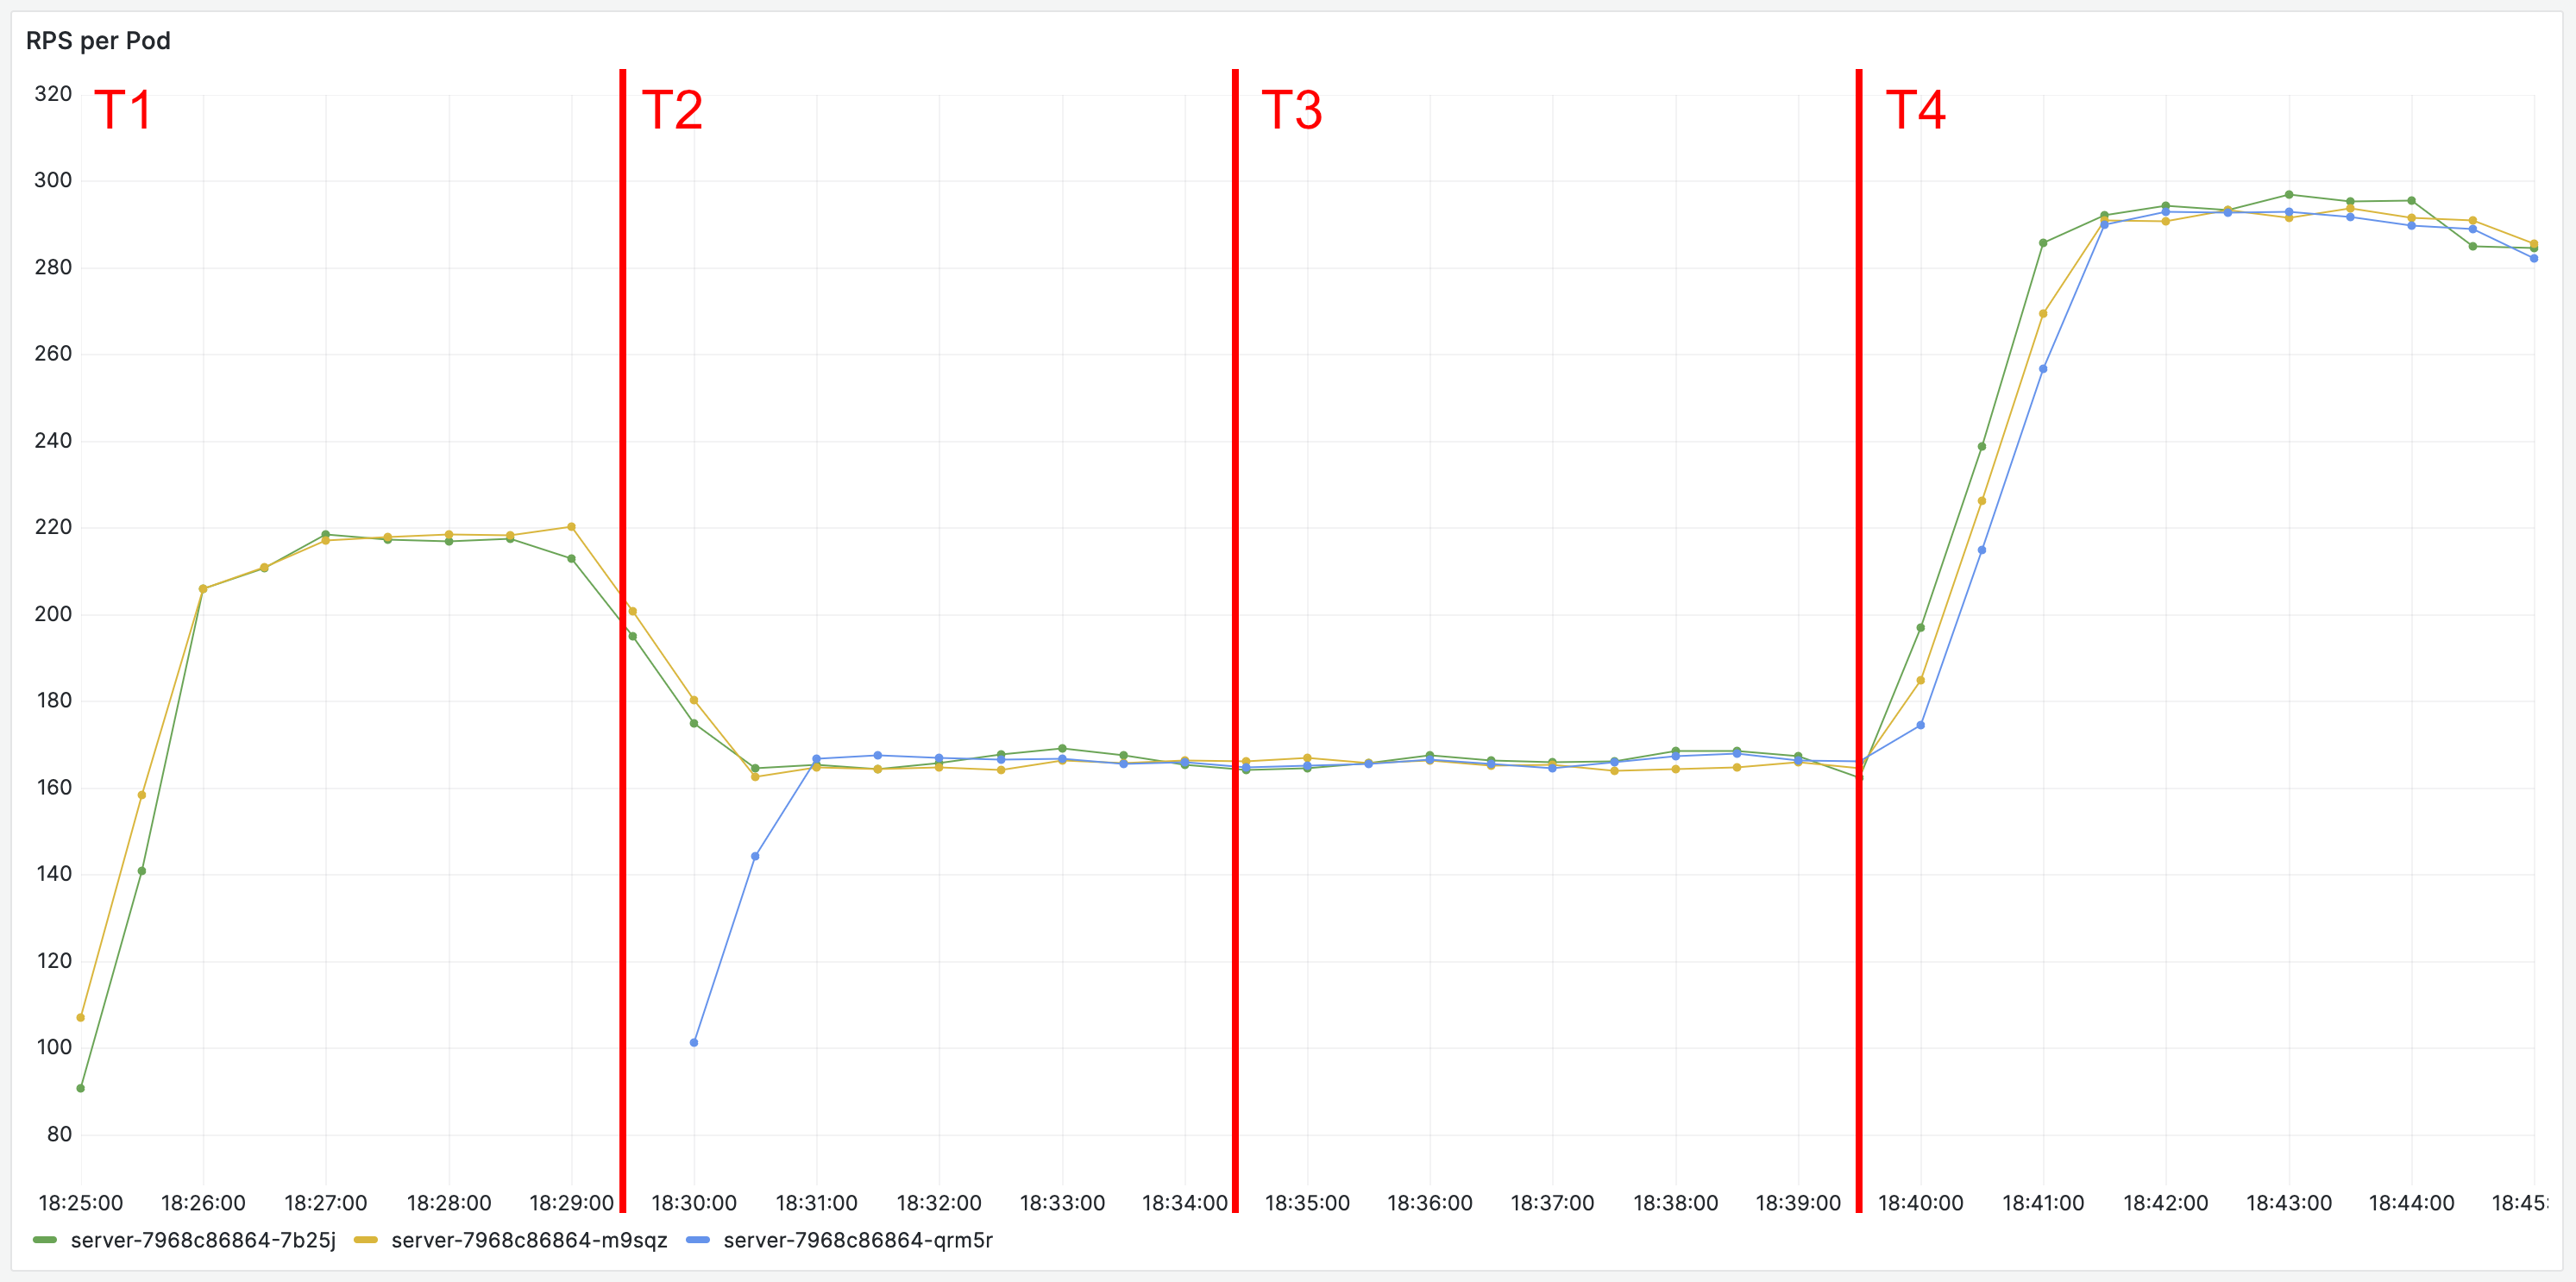
\includegraphics[width=0.75\textwidth]{img/rest_rps}
    \caption{Server RPS pro REST Pod}
    \label{fig:rest_rps}
\end{figure}

Wie an der annähernden Äquivalenz beider Graphen bis T2 in Bild~\ref{fig:rest_rps} zu erkennen ist, werden die Client-Requests von Anfang an sehr gleich auf beide Instanzen des Servers verteilt.
Sobald der Server zum Zeitpunkt T2 auf drei Instanzen skaliert wird, werden die Requests auf drei Server-Instanzen verteilt.
Dies hat eine Lastverringerung der bereits vorher zur Verfügung gestellten Server-Instanzen sowie einen in Summe erhöhten Gesamtdurchsatz zur Folge.
Der Neustart zum Zeitpunkt T3 sowie die Skalierung des Clients zum Zeitpunkt T4 haben keinen Einfluss auf die Lastverteilung der Anfragen zum Server, welche gleichbleibend gleich verteilt werden.

\begin{figure}[H]
    \centering
    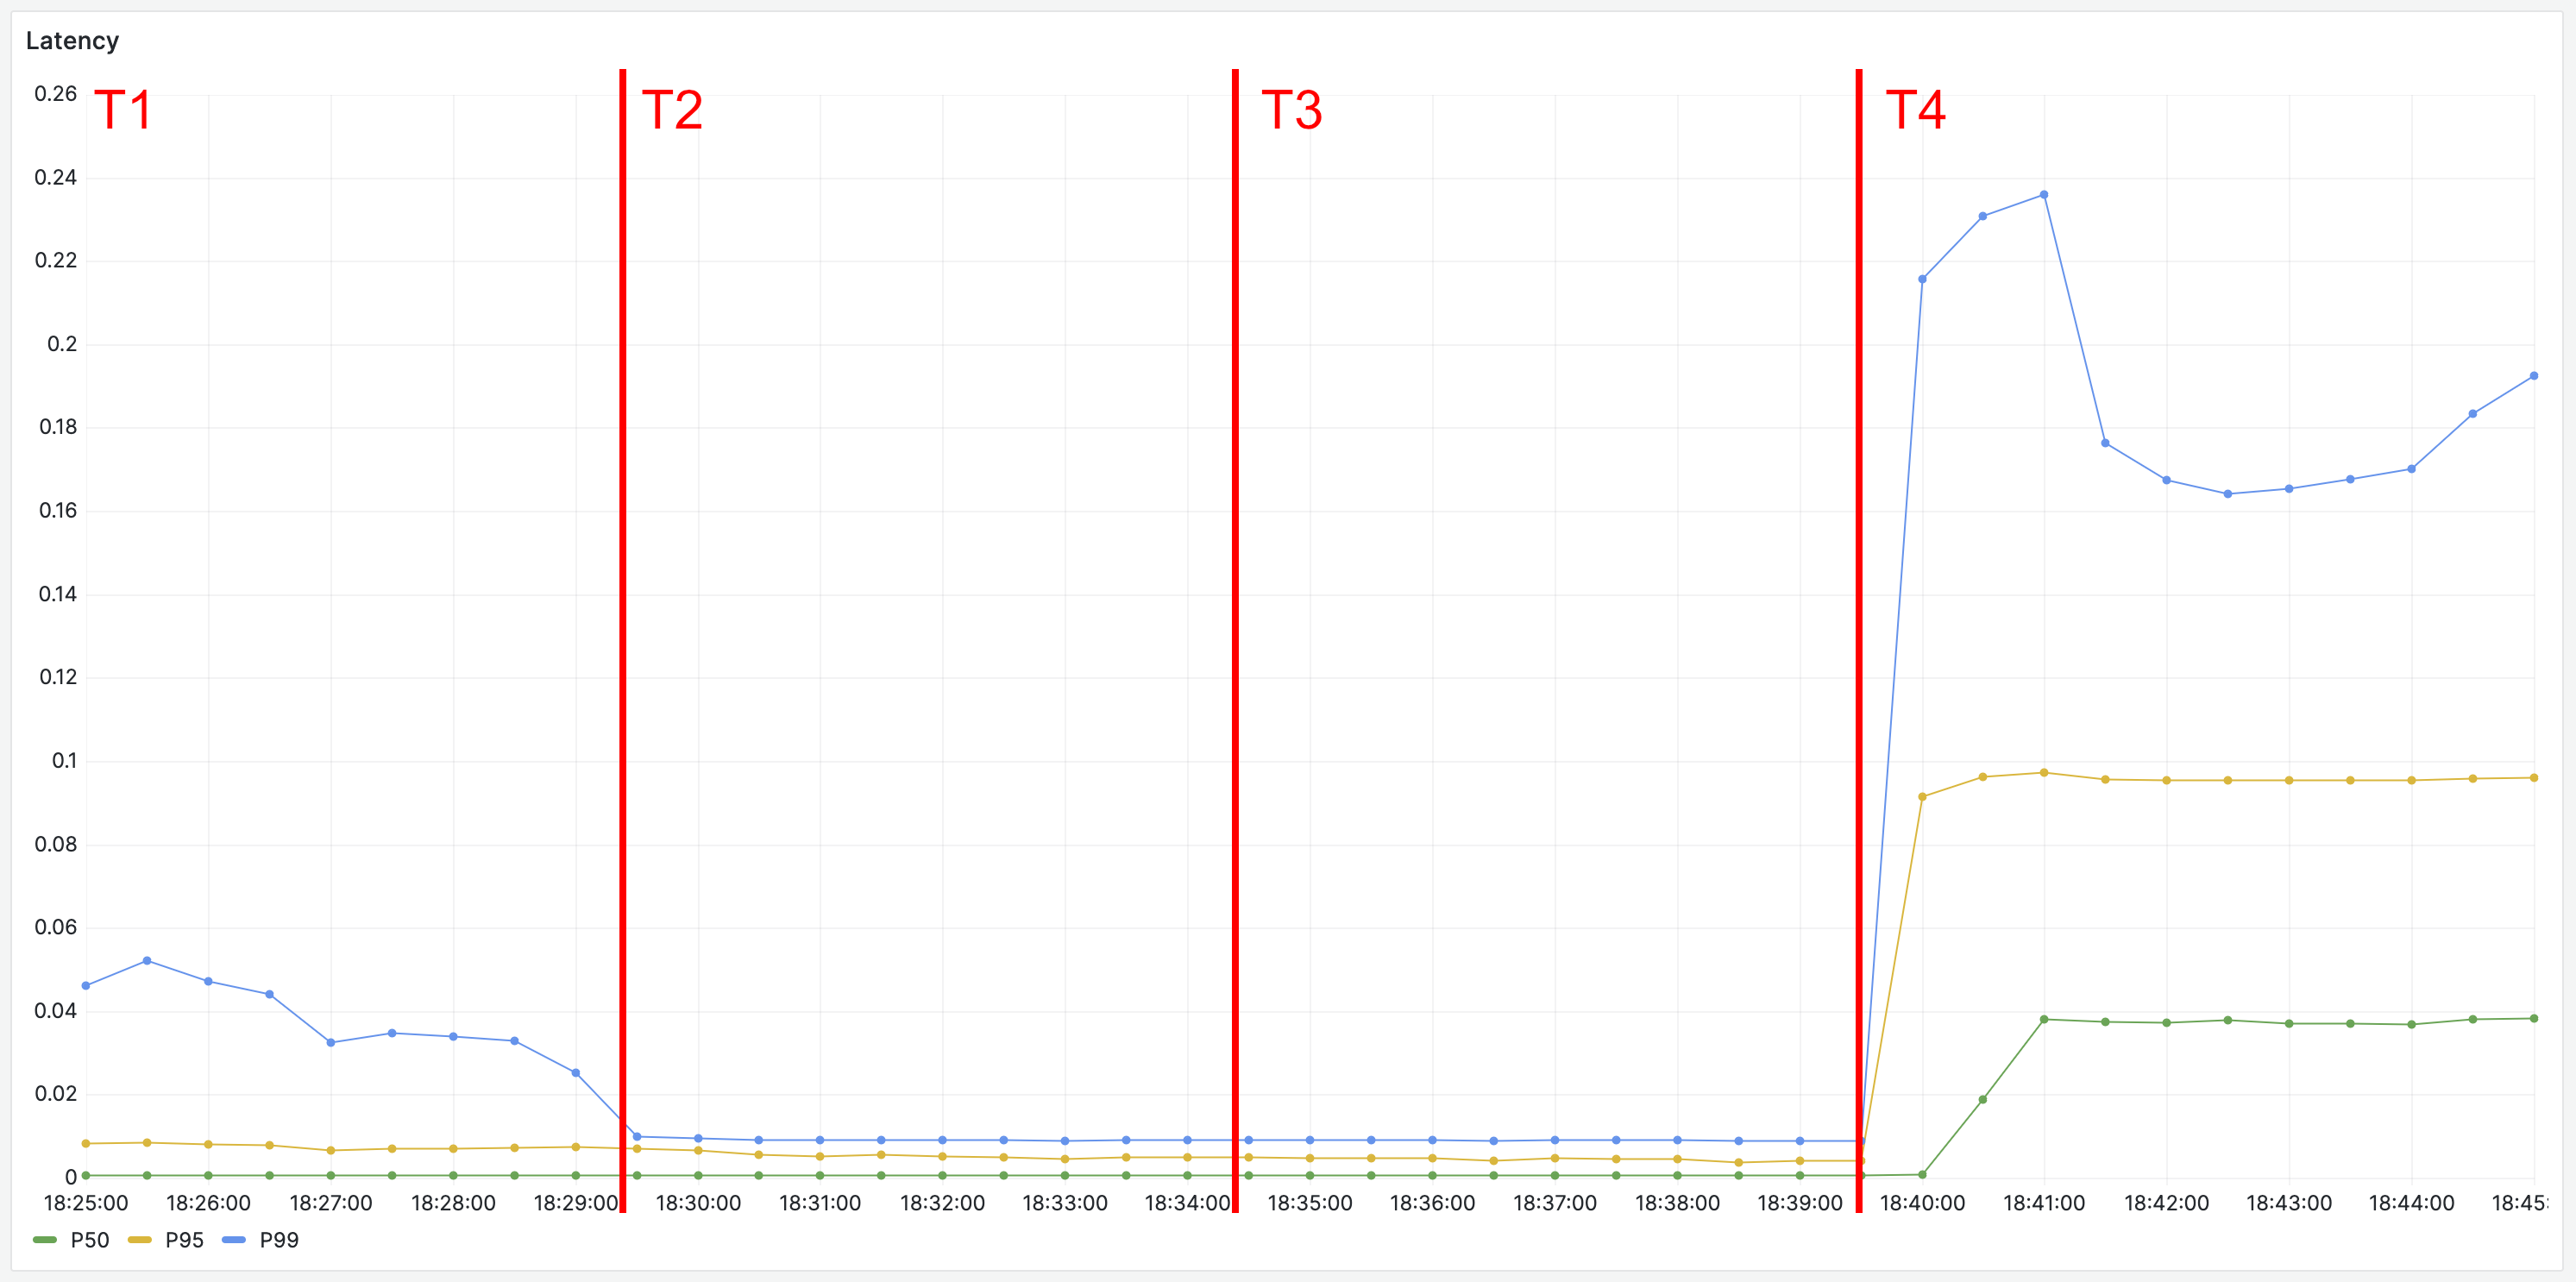
\includegraphics[width=0.75\textwidth]{img/rest_latenz}
    \caption{Rest Latenz (P99, P95, P50)}
    \label{fig:rest_latenz}
\end{figure}

Die Latenz im 99. Perzentil, gezeigt in~ Grafik\ref{fig:rest_latenz}, verbessert sich zum Zeitpunkt T2 aufgrund der nun möglichen Lastverteilung auf drei Server Instanzen, welche in Summe mehr Rechenleistung zur Verfügung haben.
Durch das hohe Aufkommen an Anfragen nach der Client-Skalierung zum Zeitpunkt T4 ist eine Verschlechterung der Latenz zu beobachten, da die Gesamtrechenleistung für den Server unangetastet bleibt.

\subsection{HTTP/2 Load Balancing}\label{subsec:http/2-load-balancing}

Nachdem nun gezeigt wurde, wie sich die Lastverteilung einer HTTP/1 Anwendung mit dem Standard Tooling von Kubernetes auswirkt, zeigt dieses Kapitel, wie sich eine Lastverteilte Anwendung, welche auf HTTP/2 basiert und sich das Standard Verhalten von Kubernetes zu Nutze macht, verhält.
An diesem Szenario werden einige Problematiken aufgezeigt, für welche in den folgenden Abschnitten nach einer Lösung gesucht wird.

\subsubsection{Standard Load Balancing}\label{subsubsec:standard}

Im Vergleich zu Szenario~\ref{subsec:http/1-load-balancing} wird die Beispielanwendung in diesem Szenario dazu konfiguriert, die gRPC-Implementierung zu verwenden.
Bis auf diesen, maßgeblichen, Unterschied, bleibt die Konfiguration identisch.

\begin{figure}[H]
    \centering
    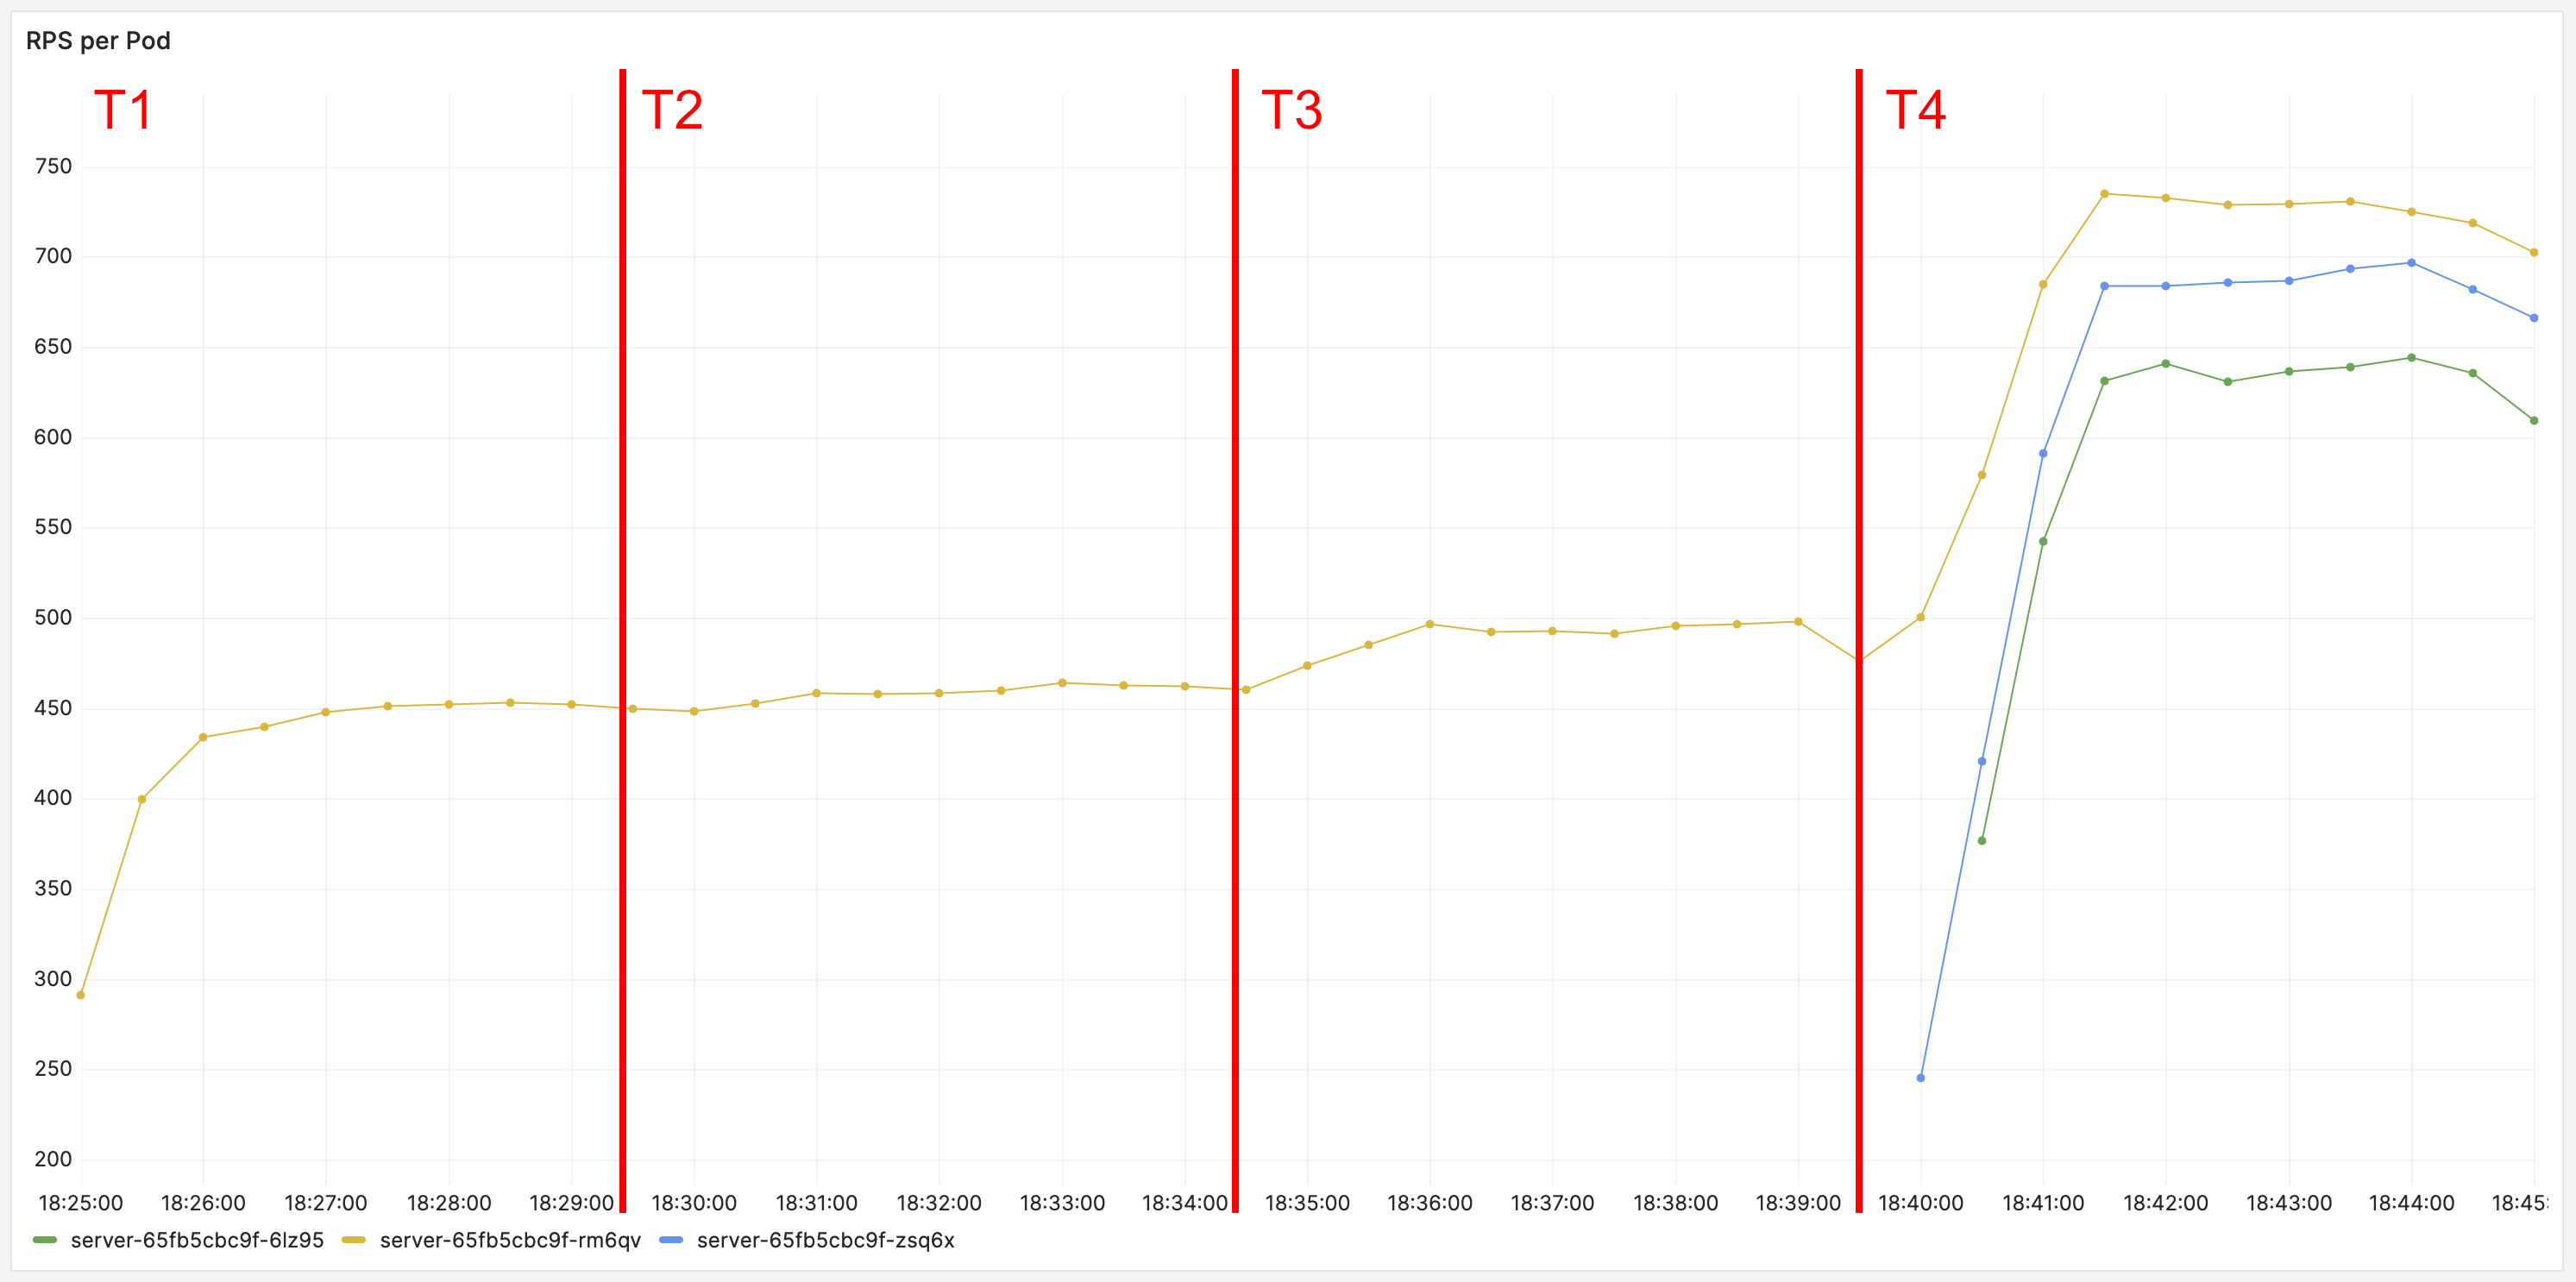
\includegraphics[width=0.75\textwidth]{img/default_rps}
    \caption{Server RPS pro HTTP/2 Standard Pod}
    \label{fig:default_rps}
\end{figure}

Grafik~\ref{fig:default_rps} spiegelt das Problem dieses Setups gut wider.
Von zeitpunkt T1 bis T4 ist zu erkennen, dass alle Requests von einem einzigen Server Pod beantwortet werden.
Diese Tatsache lässt sich damit begründen, dass HTTP/2, wie in Sektion~\ref{subsec:hyper-text-transfer-protocol} schon erwähnt, auf langlebigen Verbindungen basiert.
Zum Start des Clients wird somit eine beständige Verbindung zwischen Client und Server etabliert (siehe Bild~\ref{fig:default_loadbalancing}).
Dies hat zur Folge, dass der TCP-handshake vermieden wird und führt zu dem Problem, dass jede einzelne Anfrage über die selbe TCP Verbindung immer an die gleiche Instanz des Servers gesendet wird.

\begin{figure}[H]
    \centering
    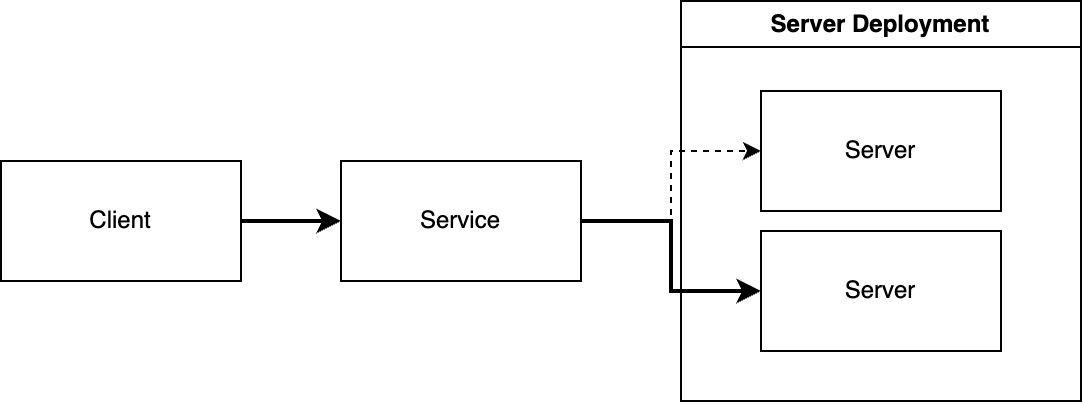
\includegraphics[width=0.75\textwidth]{img/default_loadbalancing}
    \caption{Default Implementierung Verbindungsaufbau}
    \label{fig:default_loadbalancing}
\end{figure}


Dass sich weder zum Zeitpunkt T2, noch T3 am Verhalten etwas ändert, hat hier damit zu tun, dass schlicht der gleiche Server zufälligerweise ausgewählt wird.
Da jeder Pod eine beständige Verbindung zu einem zum Startpunkt ausgewählten Server hat, kann man in diesem Fall nicht von Lastverteilung sprechen, auch wenn eine (unvorhersehbare) Verteilung der Pods auf exakt einen vorselektierten Server vollzogen wird.

Erst ab Zeitpunkt T4 werden die Anfragen der verschiedenen Clients von allen drei Servern beantwortet.
Dies hängt einfach mit der großen Anzahl der Client Pods zusammen.
Wichtig ist jedoch weiterhin, dass jeder einzelne dieser Pods immer mit genau demselben Server kommuniziert und somit keine Lastverteilung auf Request-Ebene stattfindet.


\begin{figure}[H]
    \centering
    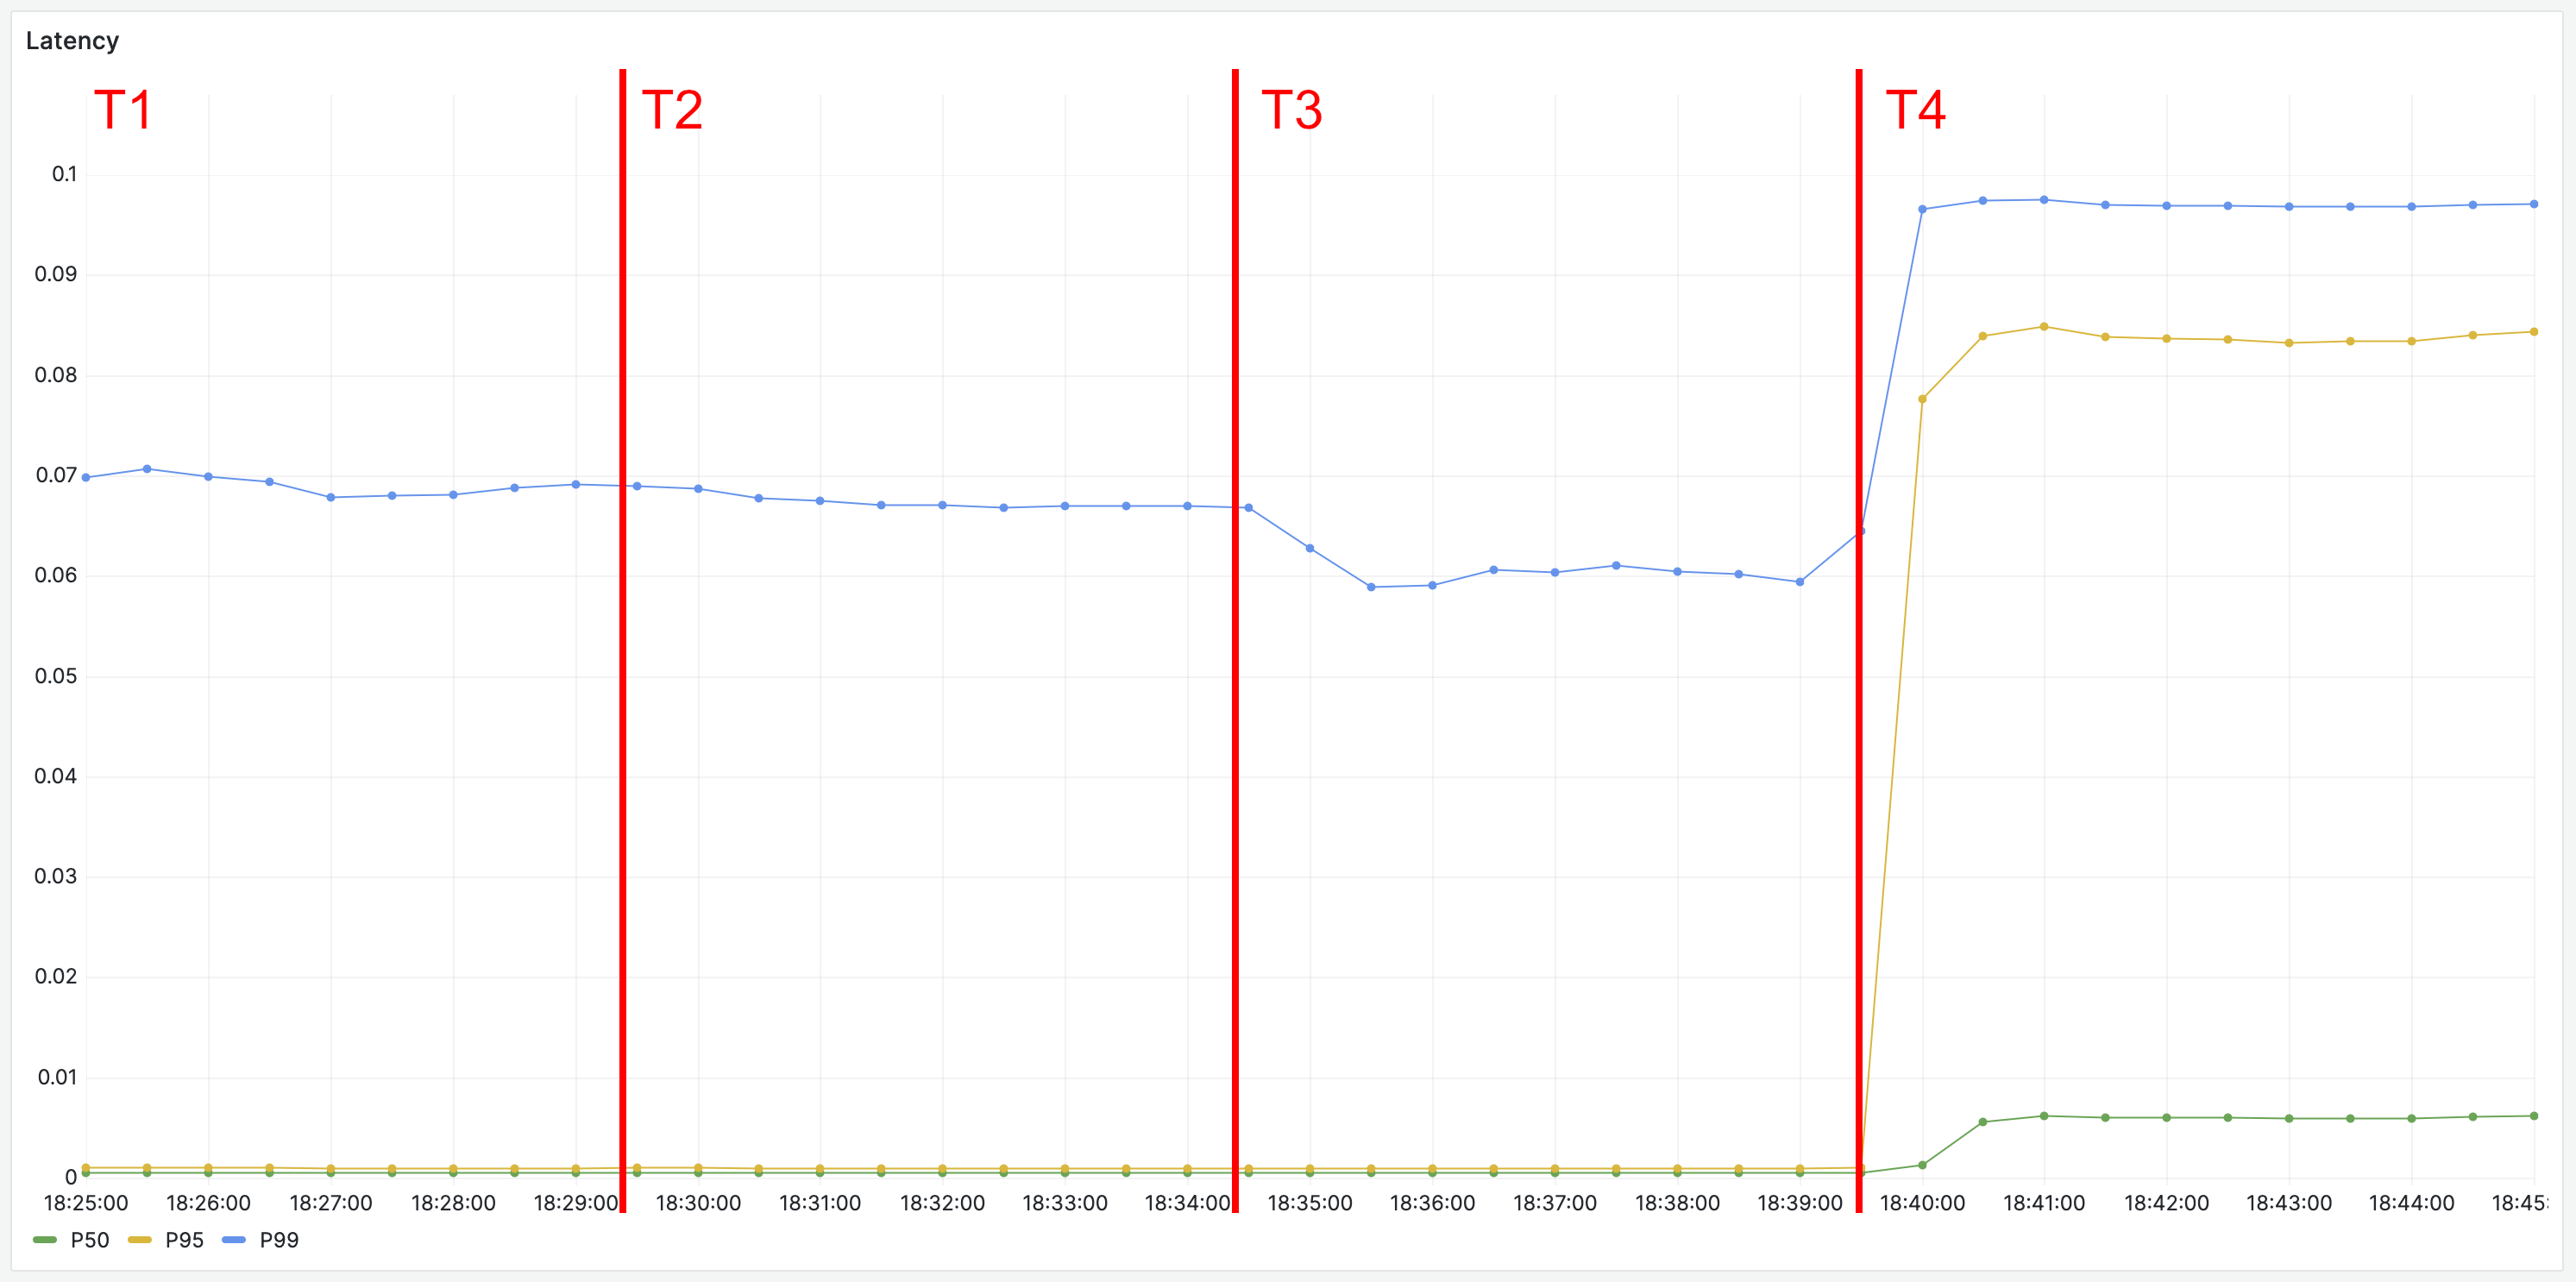
\includegraphics[width=0.75\textwidth]{img/default_latenz}
    \caption{HTTP/2 Standard Latenz (P99, P95, P50)}
    \label{fig:default_latenz}
\end{figure}

In Puncto Latenz lässt sich in Grafik~\ref{fig:default_latenz} erkennen, dass bis zu Zeitpunkt T4 keine nennenswerten Veränderungen stattfinden.

\subsubsection{Headless Service}\label{subsubsec:headless}

Nun, da gezeigt wurde, warum ein Kubernetes Service in der Standard Konfiguration keine Option zur Lastverteilung von HTTP/2-Requests ist, wird eine funktionierende Variante zur Verteilung der Requests vorgestellt.
Dieses Teilkapitel befasst sich mit Headless Services, welche unter minimalem konfigurativen Eingriff erlauben, die Last an aufkommenden HTTP/2 Anfragen auf mehrere Server Pods zu verteilen.
Listing~\ref{lst:standard} zeigt, wie ein Service des Typs ClusterIP normalerweise in einer Kubernetes Umgebung definiert wird.
Der Service erhält so eine eigene IP, welche von den Clients zentral aufgerufen wird, um auf die Replicas des Servers zuzugreifen.
Ein Namespace-Lookup auf den Service gibt hier einfach die dem Service eigens zugewiesene IP-Adresse zurück.

Im Gegensatz dazu zeigt Listing~\ref{lst:headless} die Definition eines Headless Services.
Ein Headless Service birgt die Besonderheit, dass in seiner Definition explizit angegeben wird, dass keine IP zugewiesen werden soll.
Da der Service nun keine eigene IP besitzt, werden für einen Namespace Lookup alle bekannten Pod-IPs zurückgegeben~\cite{kubernetesNetworking}.
Dieses Verhalten können wir uns im Client zunutze machen.
Zum Start des Clients werden vom Server alle bekannten IP-Adressen der Anfragen-bearbeitenden Pods geliefert.
Der Client kann nun selbst entscheiden, welcher Server zur Bearbeitung der Anfrage aufgerufen wird.
Es findet clientseitiges Loadbalancing statt.

\noindent\begin{minipage}{.45\textwidth}
             \begin{lstlisting}[caption=Standard Service,frame=tlrb,label={lst:standard}]{Name}
apiVersion: v1
kind: Service
metadata:
  name: server
  namespace: default
  labels:
    app: server
spec:
  selector:
    app: server
  ports:
    - protocol: TCP
      port: 8080
      targetPort: 8080
      name: app
             \end{lstlisting}
\end{minipage}\hfill
\begin{minipage}{.45\textwidth}
    \begin{lstlisting}[caption=Headless Service,frame=tlrb,label={lst:headless}]{Name}
apiVersion: v1
kind: Service
metadata:
  name: server
  namespace: headless
  labels:
    app: server
spec:
  selector:
    app: server
  clusterIP: None
  ports:
    - protocol: TCP
      port: 8080
      targetPort: 8080
      name: app
    \end{lstlisting}
\end{minipage}

\begin{figure}[H]
    \centering
    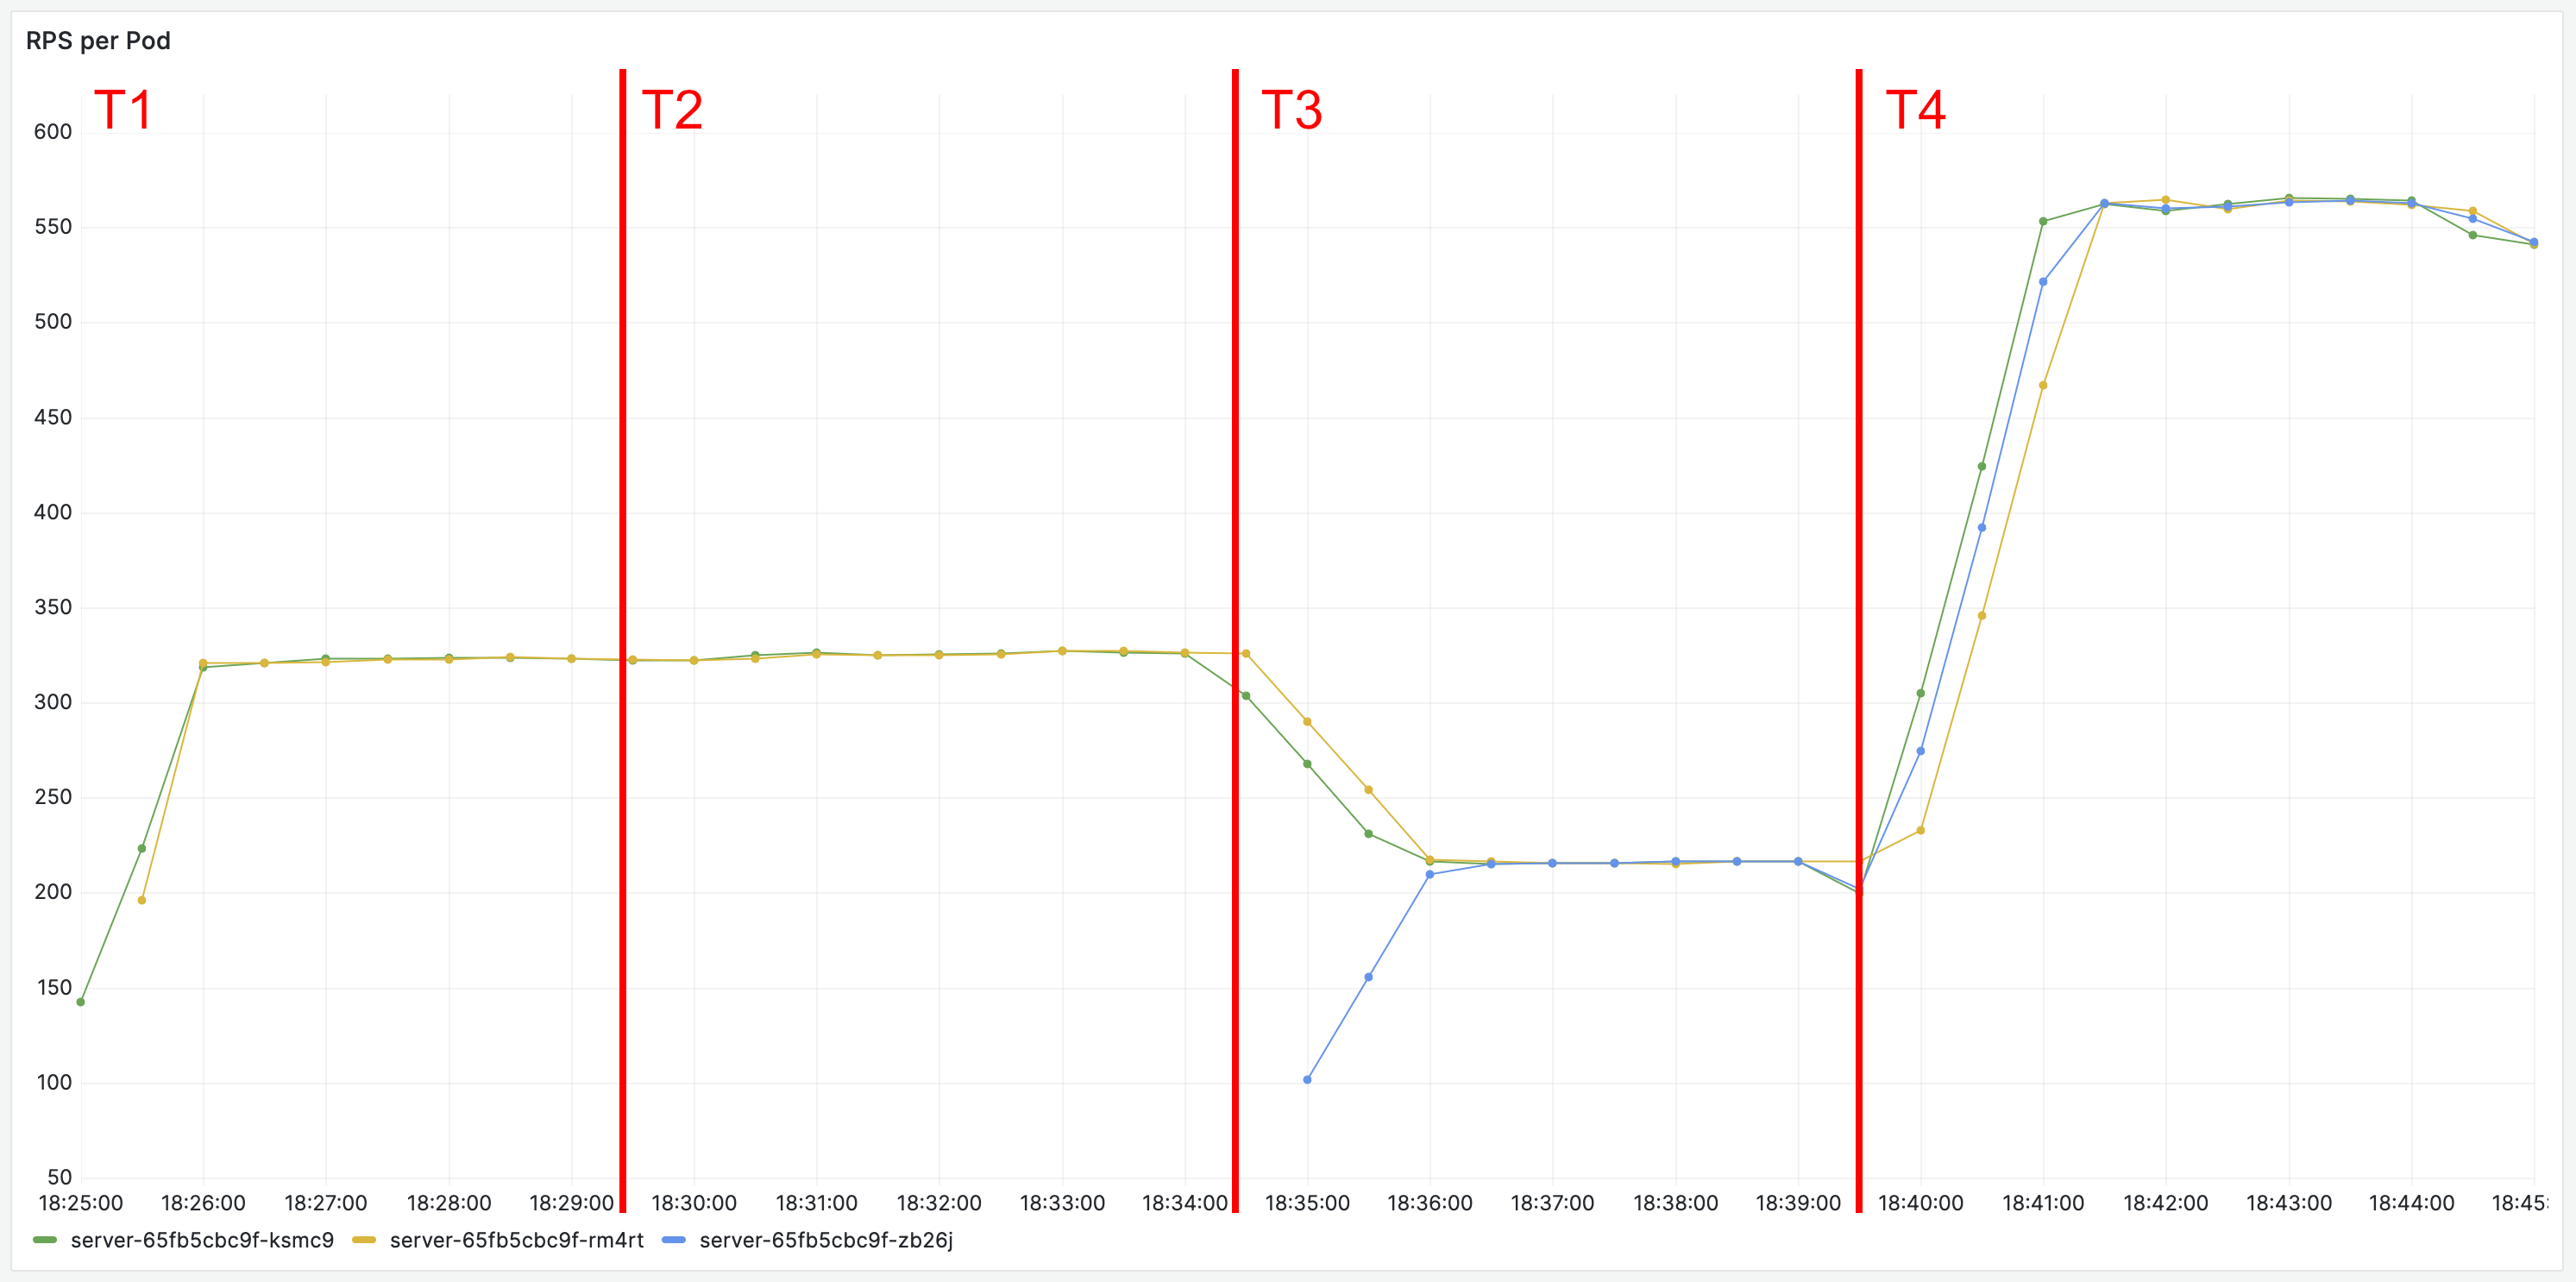
\includegraphics[width=0.75\textwidth]{img/headless_rps}
    \caption{Server RPS pro Headless Service Pod}
    \label{fig:headless_rps}
\end{figure}

Grafik~\ref{fig:headless_rps} zeigt das Anfrageaufkommen der Pods, welche über den Headless Service zur Verfügung gestellt werden.
Es ist zu erkennen, dass zu T1 mit dem Loadbalancing der Anfragen auf beide verfügbaren Instanzen begonnen wird.
Die Verteilung findet gleichmäßig statt, was sich wieder an der annähernden Äquivalenz beider Kurven erkennen lässt.
Zum Zeitpunkt T2, wenn ein neuer Server Pod hinzukommt, ändert sich nichts.
Eine Änderung ist jedoch zum Zeitpunkt T3, zu beobachten.
Dieser markiert den Neustart des Clients.
Die aufkommenden Anfragen werden jetzt gleichmäßig auf alle drei Instanzen des Servers verteilt, was einer allgemeinen niedrigeren Last pro Pod entspricht.
Das Verhalten, dass die Requests erst auf alle Server Instanzen verteilt werden, nachdem die Clients neu gestartet wurden, lässt sich mit der Funktionsweise des Headless Services erklären.

Zum Start des Clients (hier T1) werden beim Service alle verfügbaren Server IPs abgefragt (siehe 1 und 2 in Grafik ~\ref{fig:headless_loadbalancing}).
Da zu diesem Zeitpunkt die dritte Instanz noch nicht verfügbar ist, sind dem Client auch nach Skalierung des Servers weiterhin nur zwei der inzwischen drei IPs bekannt, zwischen welchen die Last per Client verteilt wird.
Auch ab Zeitpunkt T4 werden alle Anfragen weiterhin gleichmäßig auf die drei vorhandenen Server Instanzen verteilt.

\begin{figure}[H]
    \centering
    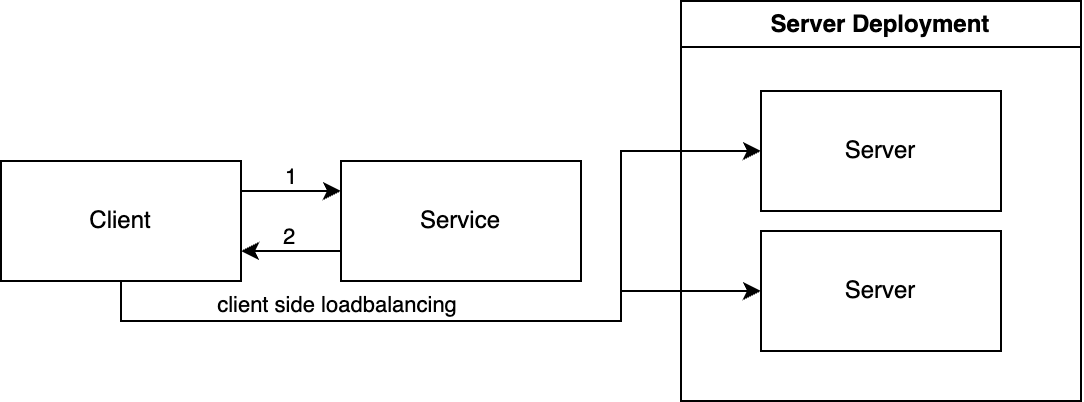
\includegraphics[width=0.75\textwidth]{img/headless_loadbalancing}
    \caption{Headless Service Client Side Loadbalancing}
    \label{fig:headless_loadbalancing}
\end{figure}

Vergleicht man Grafik~\ref{fig:headless_rps} mit Grafik~\ref{fig:default_rps}, wird schnell ersichtlich, dass die in Listing~\ref{lst:headless} gezeigte, kleine Anpassung eine große Änderung bewirkt, um das Loadbalancing von HTTP/2 Requests zu verbessern.
Zieht man jedoch die Ergebnisse in Grafik~\ref{fig:rest_rps} heran, sieht man auch, dass HTTP/1 Loadbalancing hier im Vergleich qualitativ noch immer besser funktioniert, weil die Anfragen einen neuen Server Pod sofort erreichen, sobald dessen Verfügbarkeit sichergestellt ist.

\begin{figure}[H]
    \centering
    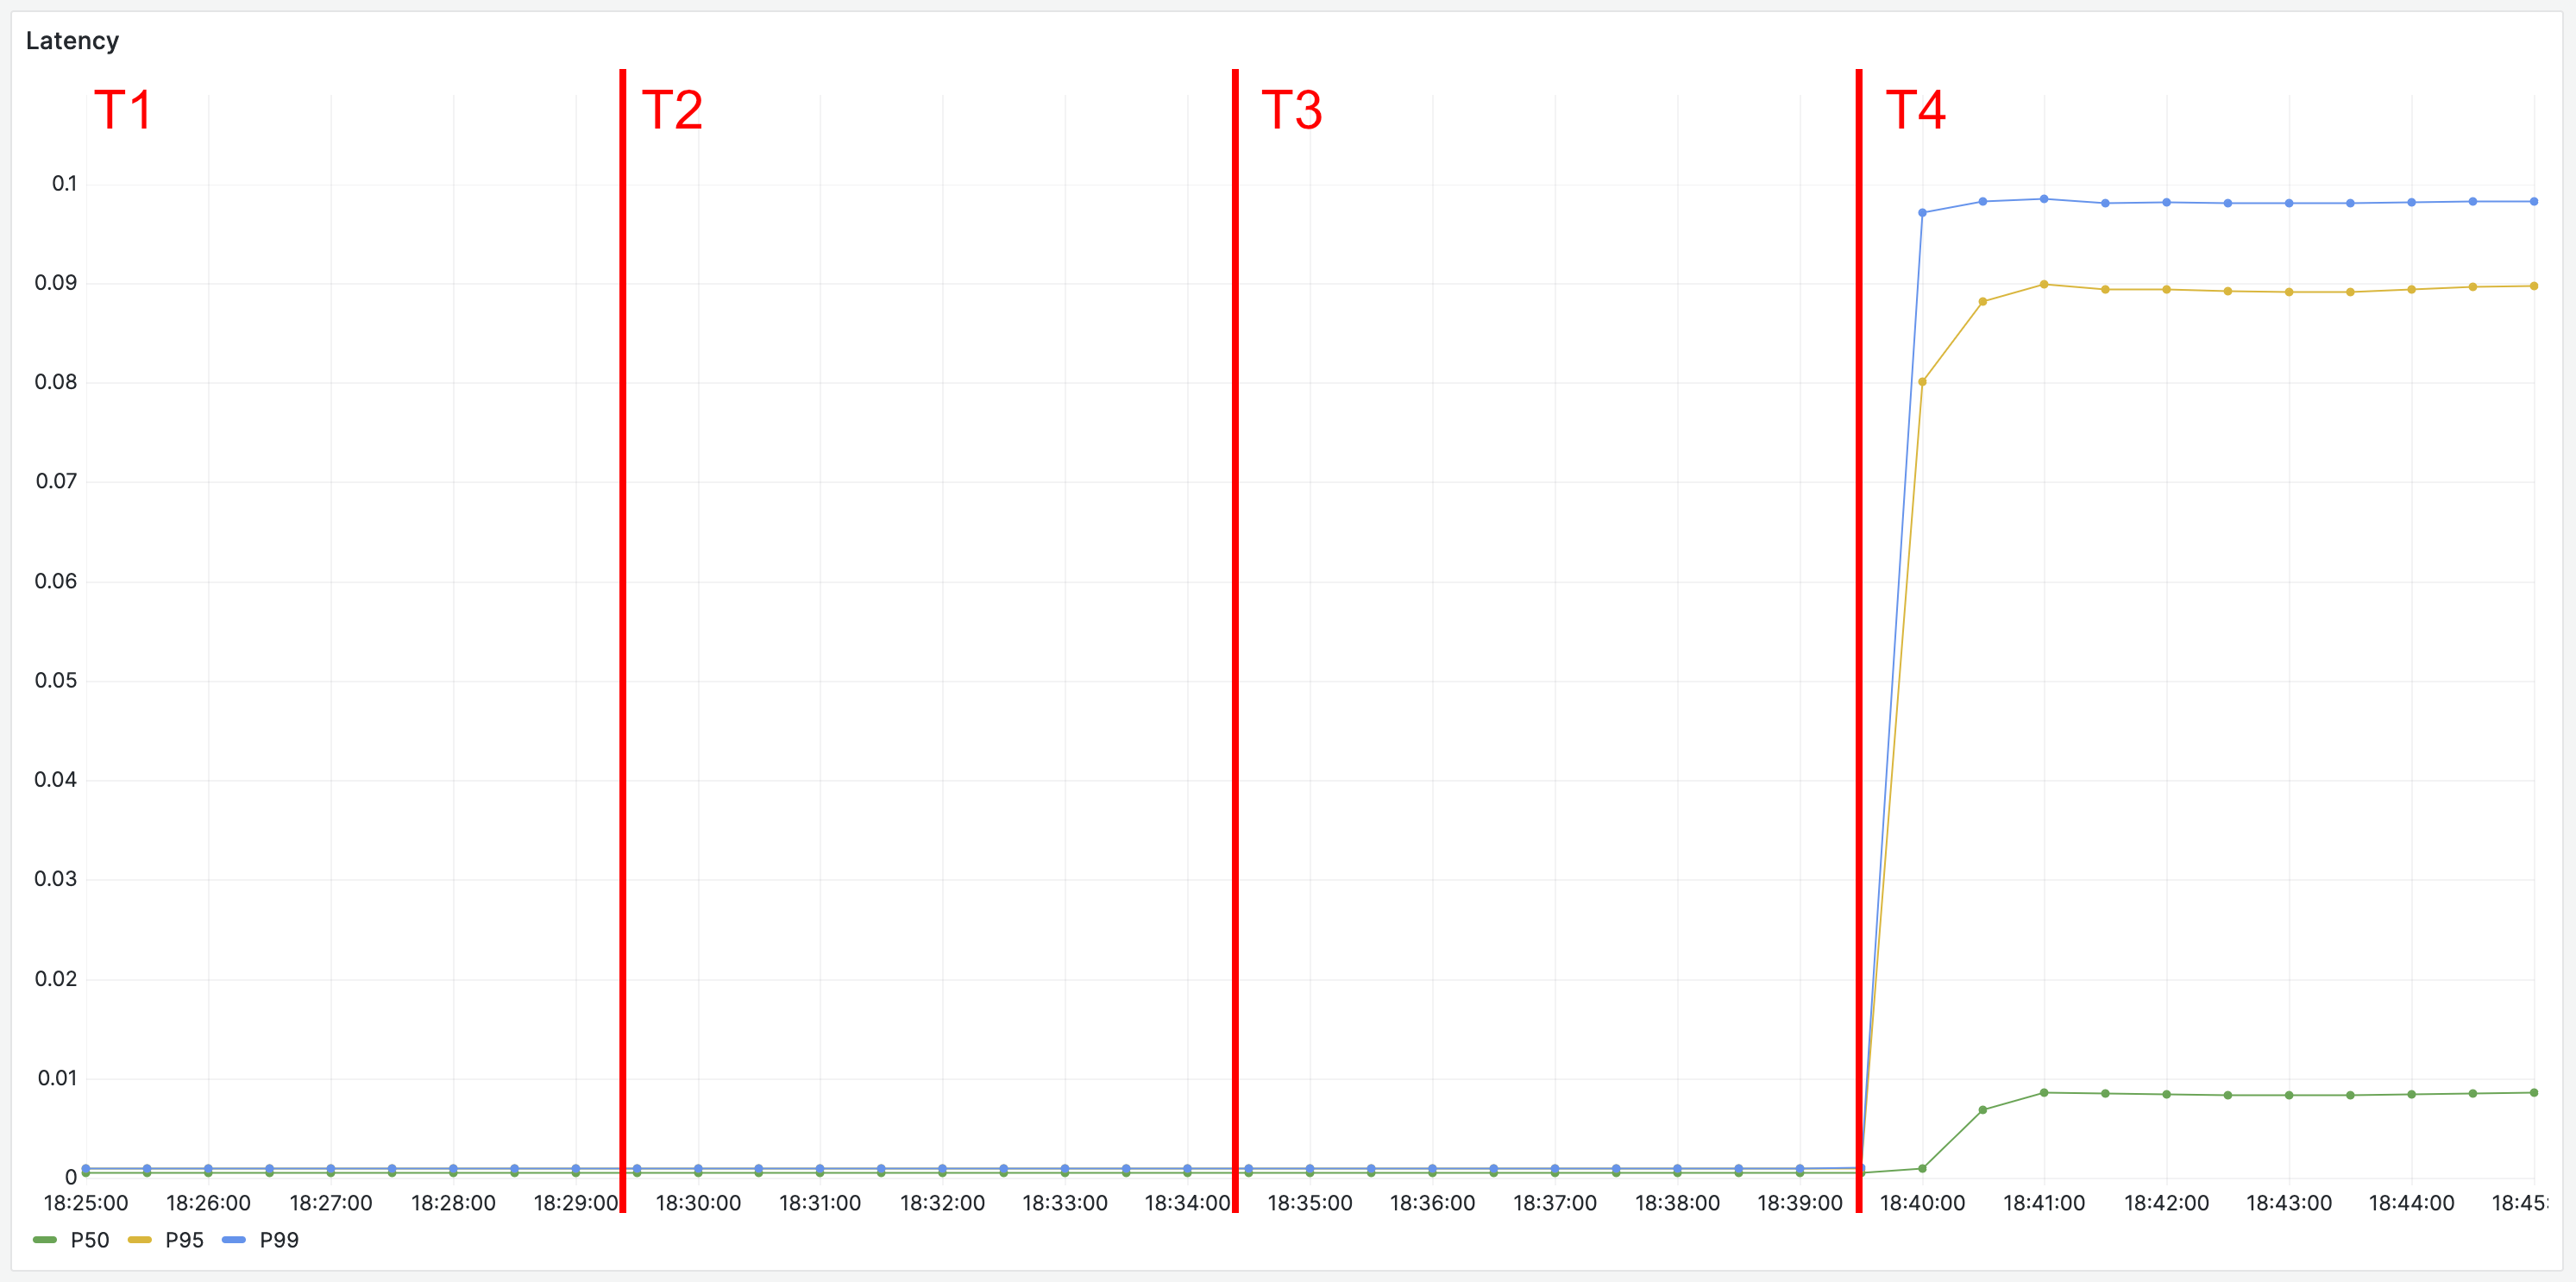
\includegraphics[width=0.75\textwidth]{img/headless_latenz}
    \caption{Headless Service Latenz (P99, P95, P50)}
    \label{fig:headless_latenz}
\end{figure}

Abbildung~\ref{fig:headless_latenz} gibt einen Überblick über die Latenzen zu diesem Szenario.
Bis zu Zeitpunkt T4 sind die Latenzen sehr unauffällig und nah beieinander.

\subsubsection{Service Mesh}\label{subsubsec:mesh}

Mit zunehmender Komplexität Cloud Nativer Anwendungen stieg der Bedarf, den Verwaltungsaufwand jener wieder zu minimieren.
Hierfür wurden Service Meshes eingeführt.
Ein Service Mesh dient als Layer zwischen Applikations- und Orchestrierungsebene und übernimmt eine Vielzahl an Aufgaben wie, für unser Szenario relevant, das Netzwerkmanagement.

Jeder Pod, welcher dem Service Mesh zugewiesen wurde, wird mit einem sogenannten Sidecar bereitgestellt.
Ein Sidecar ist ein zweiter Container innerhalb eines Pods, welcher einem bestimmten Zweck dient~\cite{koschel2021look}.
Im Falle eines Service Meshes handelt es sich um einen leichtgewichtigen Proxy server, welcher jeglichen Netzwerkverkehr unterbricht und kontrolliert.

Es gibt eine Vielzahl verschiedener Implementierungen für Service Meshes.
Aufgrund der simplen Installationsmöglichkeit wird an dieser Stelle mit LinkerD fortgefahren.
LinkerD bietet ein Command Line Interface an, welches einem hinterlegten Kubernetes Cluster die notwendigen CRDs sowie das Service Mesh selbst installiert.

Sobald das Service Mesh im Cluster installiert ist, lassen sich Pods über Annotationen zu einem Mesh zusammenfassen.
Da im vorliegenden Beispiel jeder Anwendungsfall seinen eigenen Namespace besitzt, lässt sich - wie in Listing~\ref{lst:mesh_namespace} zu sehen - über die Annotation des Namespaces einfach definieren, dass jeder beinhaltete Pod Teil des Service Meshs sein soll.

\begin{minipage}{.4\linewidth}
             \begin{lstlisting}[caption=Default Namespace,frame=tlrb,label={lst:default_namespace}]{Name}
apiVersion: v1
kind: Namespace
metadata:
  name: default
             \end{lstlisting}
\end{minipage}\hfill
\begin{minipage}{.49\linewidth}
             \begin{lstlisting}[caption=Service Mesh Namespace,frame=tlrb,label={lst:mesh_namespace}]{Name}
apiVersion: v1
kind: Namespace
metadata:
  annotations:
    linkerd.io/inject: enabled
  name: servicemesh
             \end{lstlisting}
\end{minipage}\hfill

Nachdem der Namespace annotiert wurde, können die Pods wie gewohnt über ihre Deployments bereitgestellt werden. Abbildung~\ref{fig:mesh_loadbalancing} stellt die Kommunikation zwischen Client und Server Pods im Cluster dar.
Es ist zu erkennen, dass das Verbindungsmanagement nun vollständig von den Proxies, welche als Sidecar injiziert werden, übernommen wird und jeglicher Traffic über diese geleitet wird.

\begin{figure}[H]
    \centering
    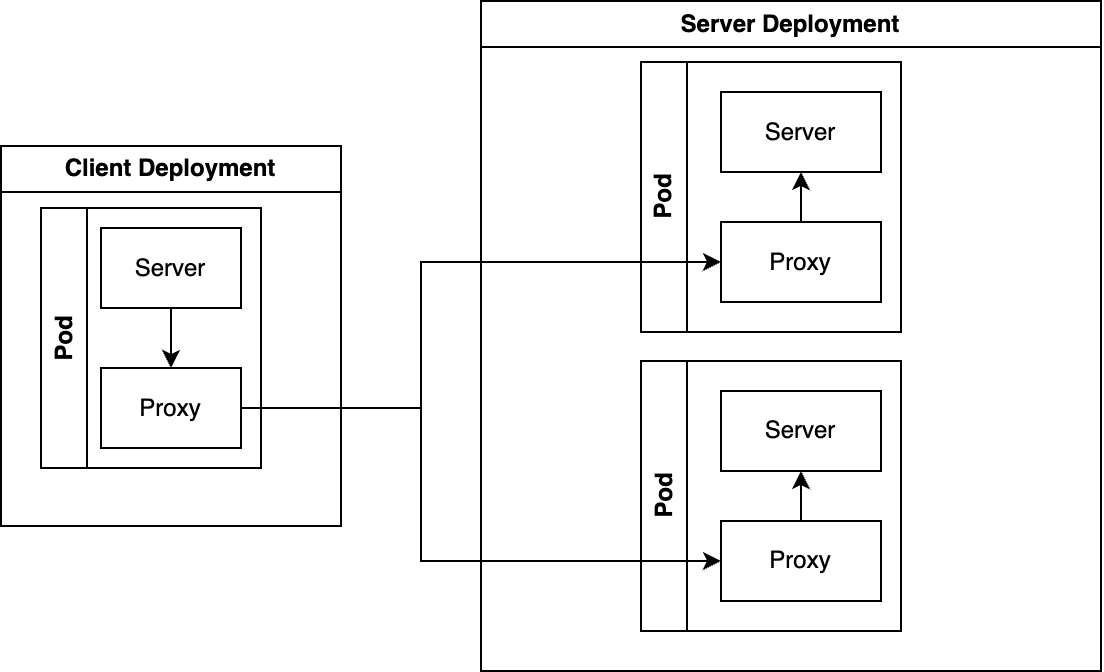
\includegraphics[width=0.75\textwidth]{img/mesh_loadbalancing}
    \caption{Connection Handling Service Mesh}
    \label{fig:mesh_loadbalancing}
\end{figure}

Wie in den vorangegangenen Kapiteln folgt eine Grafik, welche den Durchsatz der entsprechenden Implementierung pro Server Pod visualisiert.
In Grafik~\ref{fig:mesh_rps} ist zu erkennen, dass ab T1 eine Lastverteilung zwischen beiden verfügbaren Server Instanzen stattfindet.
Ab Zeitpunkt T2, welcher die Skalierung des Server Deployments auf drei Instanzen markiert, ist zu sehen, dass die Last nun auf drei Instanzen verteilt wird, eine dritte Kurve kommt hinzu.
Der Client Neustart zum Zeitpunkt T3 hat keine sichtlichen Auswirkungen auf die am Server eintreffenden Anfragen pro Sekunde.

Auch eine Erhöhung der Last durch die Skalierung des Client deployments zeigt, dass die Last weiterhin auf die vorhandenen Server Instanzen verteilt wird.

\begin{figure}[H]
    \centering
    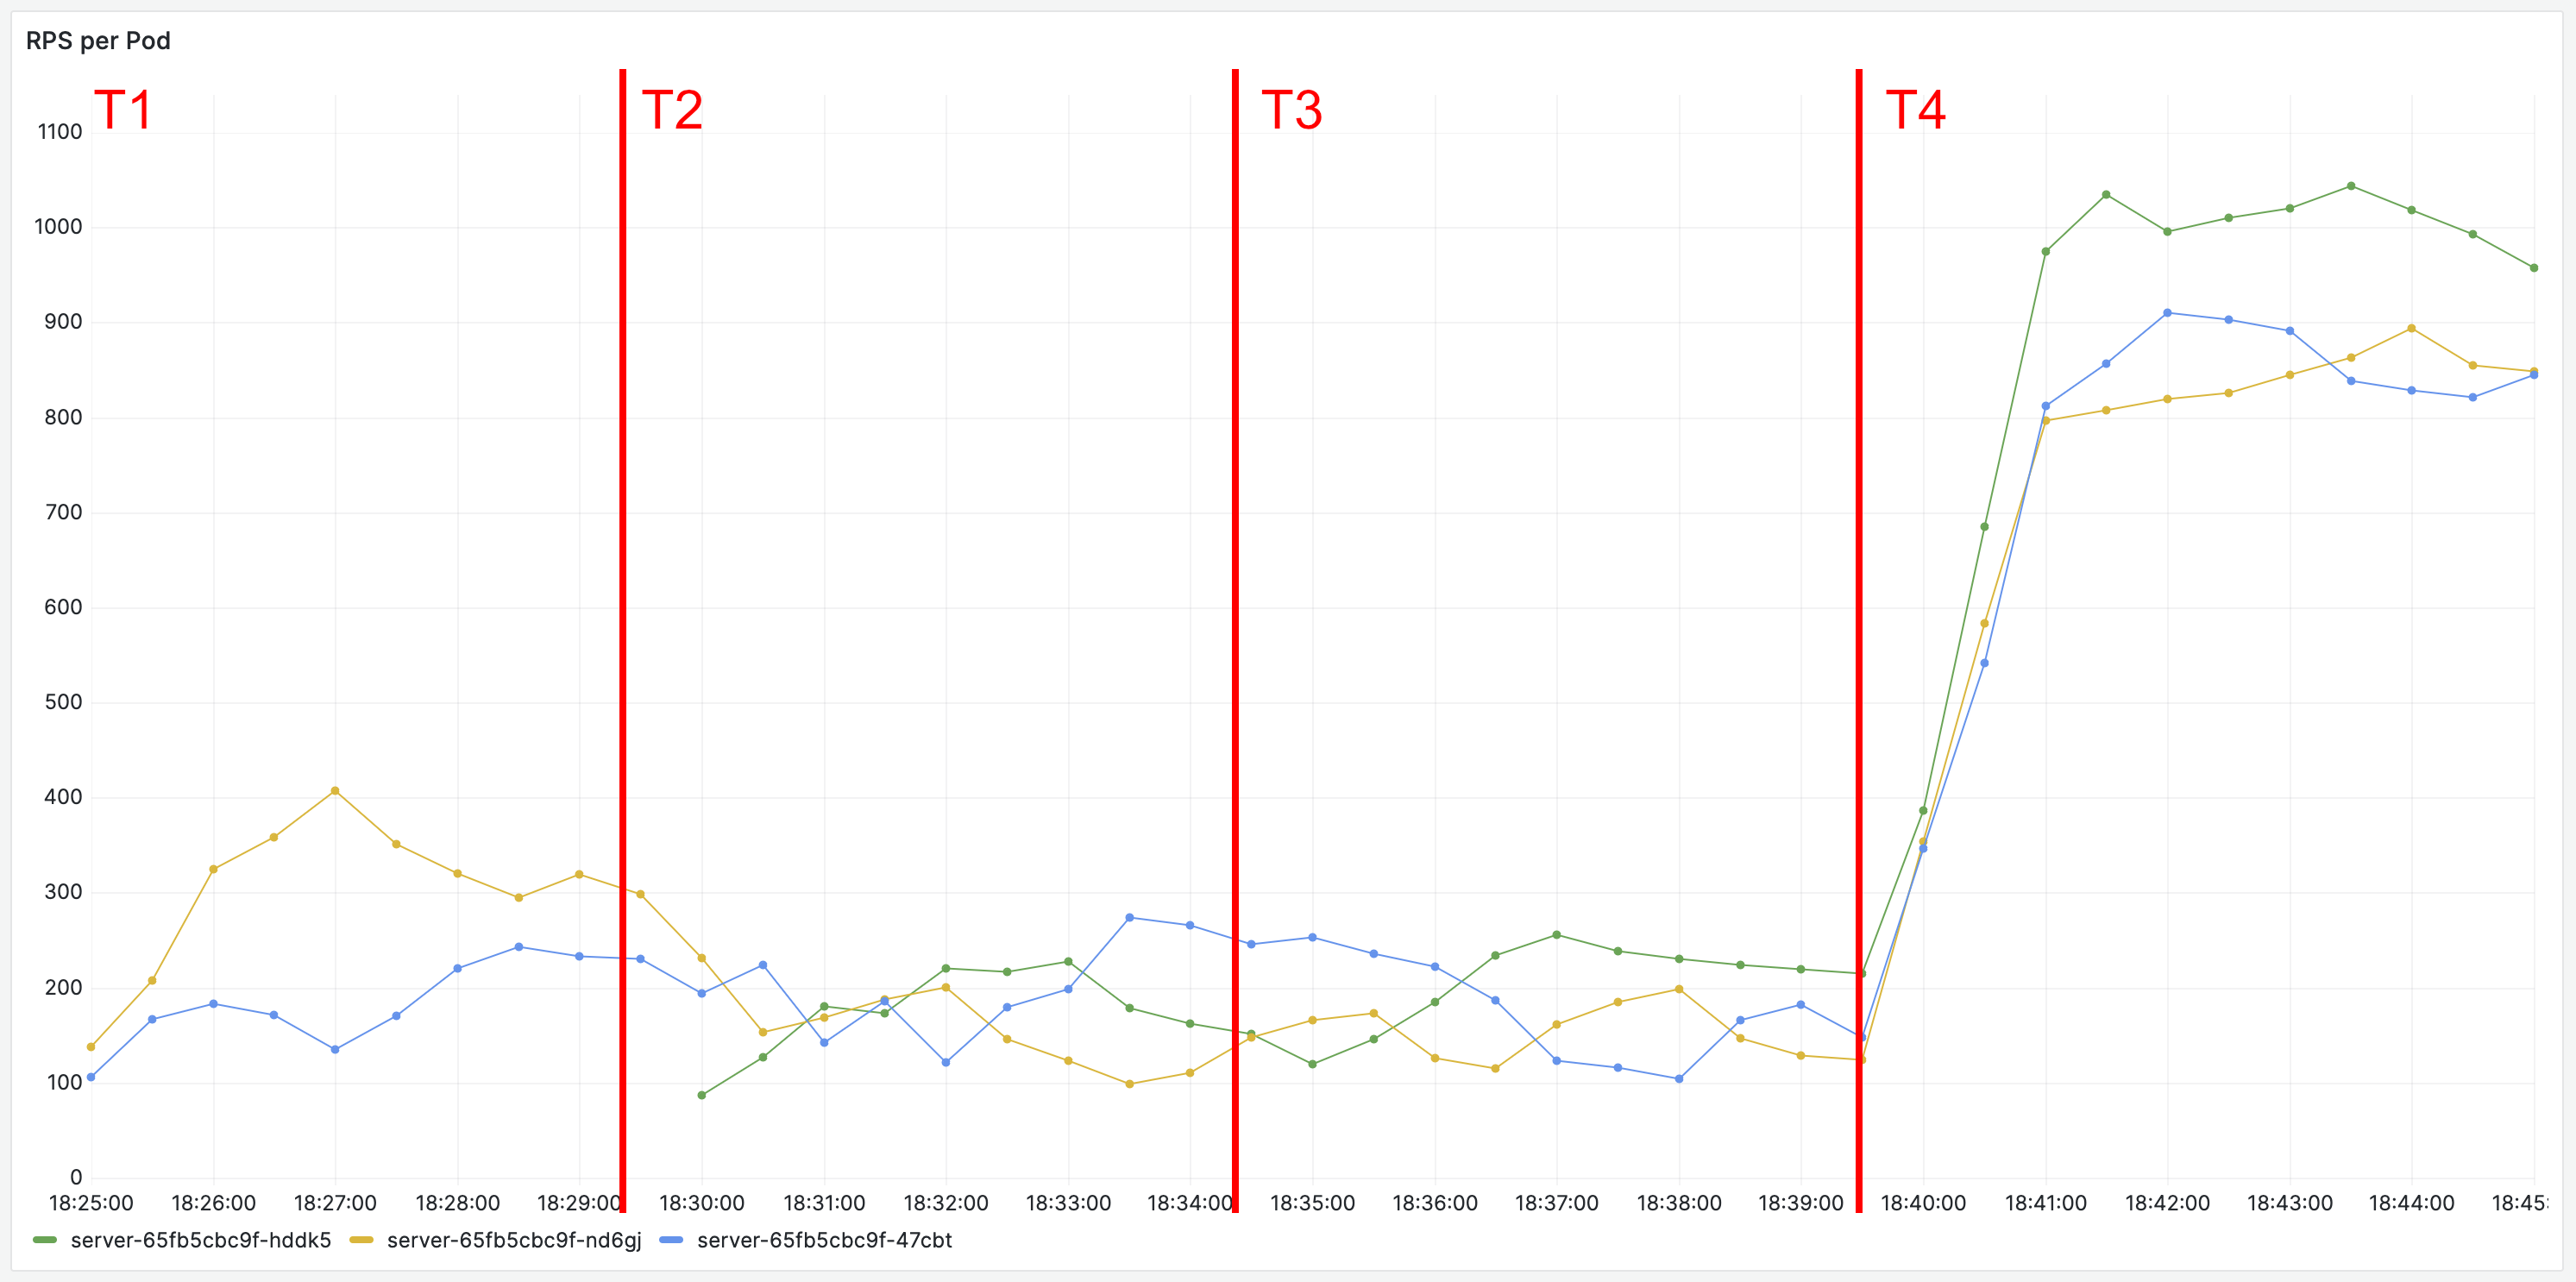
\includegraphics[width=0.75\textwidth]{img/mesh_rps}
    \caption{Server RPS pro Service Mesh Pod}
    \label{fig:mesh_rps}
\end{figure}

Grafik~\ref{fig:mesh_latenz} visualisiert die Latenz des vorgestellten Nutzungsszenarios.
Man sieht, dass die Latenz im 99. Perzentil um einiges von der im 95. Perzentil abweicht.
Ein detaillierter Vergleich der vorgestellten Metriken findet in Kapitel~\ref{sec:auswertung} statt.

\begin{figure}[H]
    \centering
    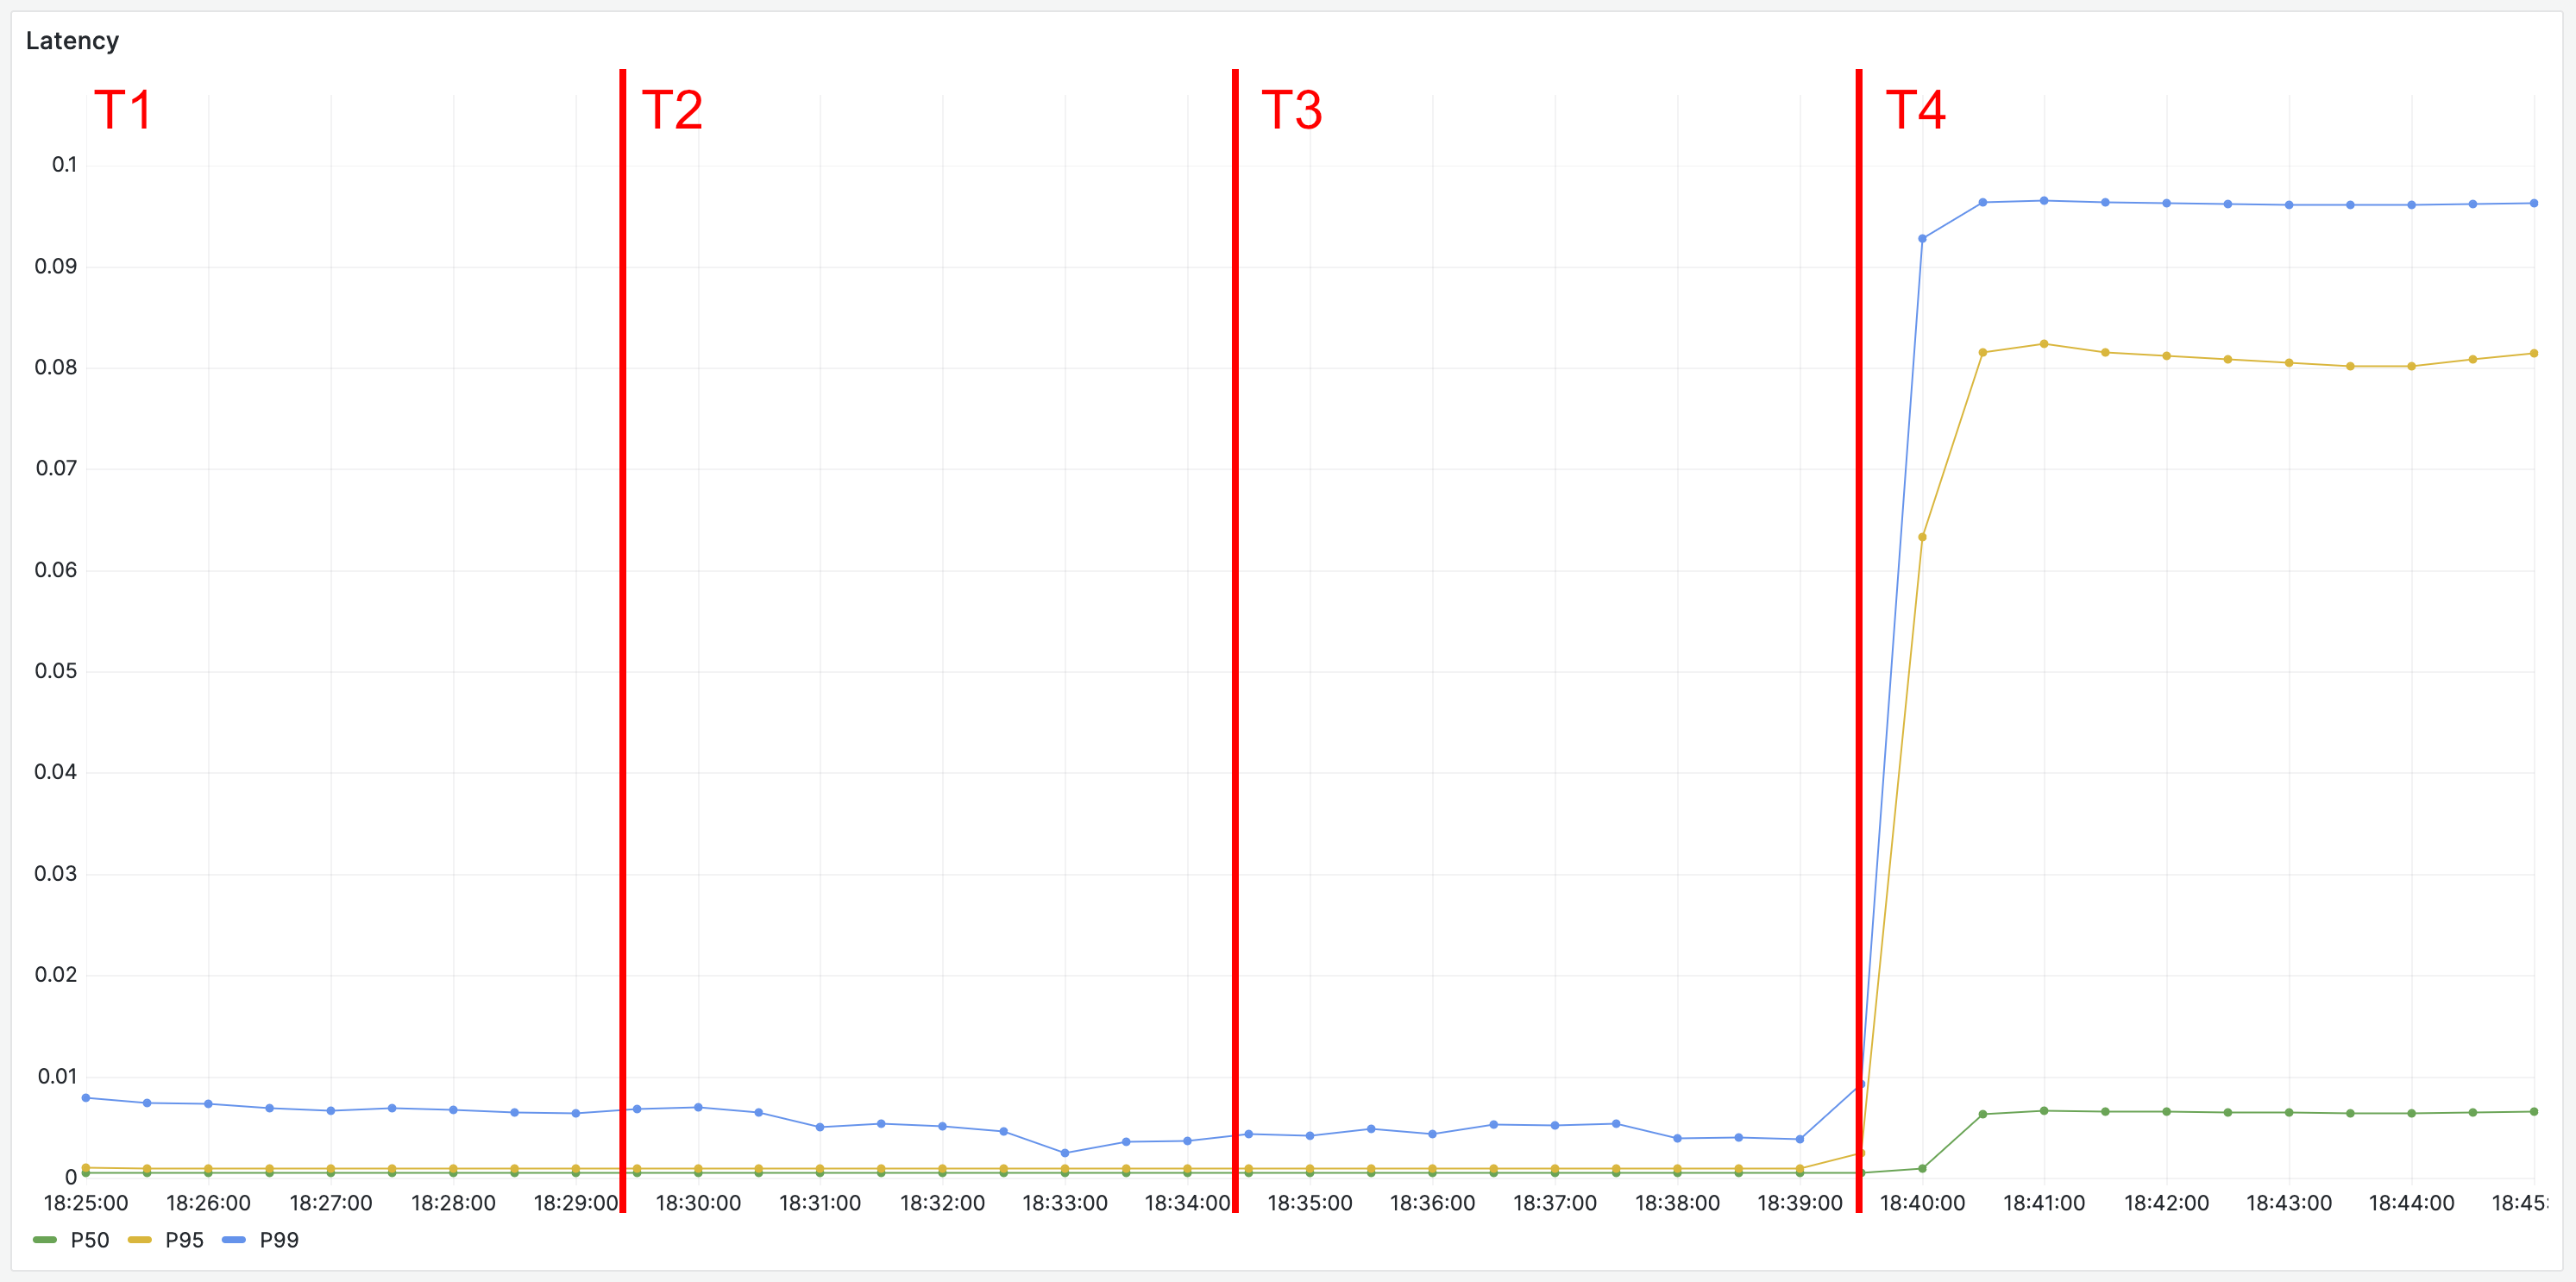
\includegraphics[width=0.75\textwidth]{img/mesh_latenz}
    \caption{Service Mesh Latenz (P99, P95, P50)}
    \label{fig:mesh_latenz}
\end{figure}

\newpage


\section{Auswertung}\label{sec:auswertung}

Das folgende Kapitel beschäftigt sich mit der Auswertung der in den vorangegangen Kapiteln vorgestellten Metriken.
Zu Beginn wird auf die Fairness der verschiedenen Implementierungen eingegangen.
Anschließend werden die verschiedenen vorgestellten Varianten der Bereitstellung auf ihre Performance hin untersucht.
Abschließend wird die Nutzbarkeit der Lösungen verglichen.
Hier spielen weniger Metriken als Qualitätsmerkmale der Lösungen zur Nutzbarkeit in der Praxis eine Rolle.

\subsection{Fairness}\label{subsec:fairness}

Fairness spielt in Hinblick auf Skalierbarkeit eine große Rolle und ist eine notwendige Bedingung für die Erreichbarkeit guter Performance.
Ohne ein faires Loadbalancing kann nicht sichergestellt werden, dass jede Instanz eines Deployments bestmöglich ausgelastet werden kann.

Um die Fairness zu bewerten, genügt es zu beobachten, wie viele Anfragen jede Instanz in einem gegebenen Zeitraum erreichen.
Da zum Zeitpunkt T2 eine Skalierung des Server Deployments stattfindet, wird der Zeitraum T2 bis Ende herangezogen.
Auf Basis der Metrik, welche auch für den Durchsatz (RPS) herangezogen wird, ergibt sich Tabelle~\ref{tab:requests}.

\begin{table}[H]
    \centering
    \begin{tabular}{|l|l|l|l|l|}
        \hline
        & Pod 1  & Pod 2  & Pod 3  & Standardabweichung \\ \hline
        REST     & 265.757 & 262.532 & 194.967 & 32.637,153          \\ \hline
        Standard & 198.091 & 665.355 & 224.484 & 214.320,496         \\ \hline
        Headless & 451.578 & 440.857 & 245.620 & 94.663,805          \\ \hline
        Mesh     & 446.578 & 467.815 & 467.573 & 9.954,668           \\ \hline
    \end{tabular}
    \caption{Durchsatz pro Pod und Standardabweichung}
    \label{tab:requests}
\end{table}

Tabelle~\ref{tab:requests} zeigt, wie viele Anfragen jeder Pod pro Variante im Zeitraum von T2 bis zum Messende erhalten hat.
Auf Basis dieser Werte wird die Standardabweichung berechnet.
Es ist zu erkennen, dass die Umsetzung über das Service Mesh mit einer Standardabweichung von 9.954,668 Anfragen am fairsten ist.
An dieser Stelle ist zu erwähnen, dass diese Variante die einzige unter den HTTP/2 Loadbalancing Implementierungen ist, welche sogar fairer ist, als das Kubernetes Standard Loadbalancing von HTTP/1 Anfragen mit einer Standardabweichung von 32.637,153 Anfragen.
Gefolgt wird es von der Headless Implementierung mit 94.663,805 und der Standard HTTP/2 Implementierung mit 214.320,496 abweichenden Anfragen.

\subsection{Performance}\label{subsec:performance}

Die Performance kann anhand zweier Metriken gemessen werden.
Diese Metriken betreffen zum einen den serverseitig messbaren Durchsatz sowie die clientseitig messbare Latenz, also die Dauer von Absetzen der Anfrage bis zum Empfang der entsprechenden Antwort.

\subsubsection{Durchsatz}

Serverseitig wird hier beobachtet, wie viele Anfragen das Deployment in Summe beantworten konnte, es wird also der gesamte Durchsatz auf den definierten Zeitraum verglichen.
Wie in Sektion~\ref{subsec:fairness} bereits beschrieben, ist es auch hier sinnvoll, nur den Zeitraum von T2 bis zum Messende zu betrachten.

\begin{table}[H]
    \centering
    \begin{tabular}{|l|l|}
        \hline
        & Durchsatz \\ \hline
        REST     & 723.256    \\ \hline
        Standard & 1.087.930   \\ \hline
        Headless & 1.138.055   \\ \hline
        Mesh     & 1.381.966   \\ \hline
    \end{tabular}
    \caption{Gesamtdurchsatz}
    \label{tab:durchsatz}
\end{table}

Tabelle~\ref{tab:durchsatz} gibt hier einen Überblick über die ermittelten Werte.
Schon am Vergleich zwischen REST und Standard ist eine erhöhung des Durchsatzes erkennbar, auch wenn Sektion~\ref{subsec:fairness} ergeben hat, dass die Standard Implementierung die unfairste ist.
Dies hat den Hintergrund, dass der TCP Handshake, welcher einen zeitlichen Aufwand bedeutet, durch die Beständigkeit der HTTP/2-Verbindungen von der Anzahl aller Requests reduziert werden kann auf die Anzahl der Clients.
Da die Implementierungen Standard, Headless und Mesh auf dem gleichen Protokoll aufbauen, ist ein Vergleich hier besser angebracht.
Es lässt sich eine Korrelation zur Fairness erkennen, indem die Mesh Implementierung, welche am fairsten ist, auch den höchsten Durchsatz aufweist.
Gefolgt wird diese Implementierung von der Headless, welche - ungeachtet der REST-Implementierung - am zweit fairsten ist.

\subsubsection{Latenz}
Clientseitig ergibt sich die Möglichkeit, das Ergebnis anhand seiner Latenzen zu vergleichen.
Hier ist es sinnvoll, die Latenzen in dem Zeitraum zu betrachten, in dem das System der höchsten Last ausgesetzt war.
Dies trifft auf den Zeitraum T4 bis zum Messende zu, da hier durch die Skalierung des Clients auf 30 Pods am meisten Netzwerk-Traffic generiert wurde.

\begin{table}[H]
    \centering
    \begin{tabular}{|l|l|l|l|}
        \hline
        & Ø-P50 & Ø-P95 & Ø-P99 \\ \hline
        REST     & 0,032 & 0,095 & 0,179 \\ \hline
        Standard & 0,005 & 0,083 & 0,097 \\ \hline
        Headless & 0,007 & 0,088 & 0,098 \\ \hline
        Mesh     & 0,005 & 0,079 & 0,096 \\ \hline
    \end{tabular}
    \caption{Durchschnittliche Latenzen über den Zeitraum T4 bis ende}
    \label{tab:latenz}
\end{table}

Tabelle~\ref{tab:latenz} gibt zu erkennen, dass jede gRPC-Implementierung im Vergleich zur REST Implementierung eine deutlich niedrigere Latenz aufweisen kann.
Vergleicht man innerhalb dieser Implementierungen die Latenzen miteinander, so lässt sich erkennen, dass Headless minimal langsamer ist als die Standard Implementierung.
Das hängt vermutlich mit dem client seitigen Loadbalancing zusammen, das den angesprochenen Server auswählt, was bei der Standardimplementierung wegfällt.
Schneller als die Standard Implementierung ist noch die Mesh Implementierung.
Da jedoch die Latenz Unterschiede im Allgemeinen sehr gering sind, können diese vernachlässigt werden und spielen im Vergleich zum Durchsatz und der Fairness eine eher untergeordnete Rolle.

\subsection{Nutzbarkeit}\label{subsec:nutzbarkeit}

Alle Implementierungen wurden nun inwelcher den Neustart der Client Pods markiert Bezug auf ihre Performanz bewertet.
Neben der Performance ist aber auch die Nutzbarkeit ein wichtiger Aspekt.
So kann nicht jede Implementierung für jedes Nutzungsszenario empfohlen werden.
Daher folgt eine kurze Nutzbarkeitsbewertung nicht-quantitativer Eigenschaften.

\subsubsection{Standard}
Die Standard Implementierung sollte aufzeigen, warum verschiedene Ansätze des Loadbalancings für HTTP/2 Applikationen betrachtet werden.
Im Allgemeinen ist diese Umsetzung nicht für den Produktivgebrauch zu empfehlen, da sie nur mit der Anzahl der Clients skaliert.
Automatische Skalierung der Server im Falle eines erhöhten Anfrageaufkommens wäre Sinnlos, da nur neue Clients eine Verbindung zu neuen Server Instanzen herstellen können, was auch eher dem Zufall überlassen wird.

\subsubsection{Headless}
Diese Umsetzung ermöglicht das client seitige Load Balancing.
Clients rufen zu Beginn alle adressierbaren IPs über den Headless Service ab und verteilen die Last dann im Round Robin verfahren selbst.
Vorteil gegenüber dem Standard verfahren ist, dass Loadbalancing zumindest zwischen allen bekannten Server Instanzen stattfindet.
Nachteil an dieser Umsetzung ist, ähnlich dem Nachteil der Standard Umsetzung, dass sie nicht unbedingt serverseitig skalierbar ist.
Wenn eine neue Server Instanz zur Verfügung gestellt wird, wird diese nur von CLients angesprochen, welche nach der neuen Server Instanz provisioniert werden.
Daher eignet sich diese Variante besonders für den Anwendungsfall, dass der Server gar nicht automatisch skaliert werden soll bei last, sondern stets in einer festen Replicagröße provisioniert ist.
Das liegt daran, dass sie abgesehen von der Modifikation des Services, keinerlei Mehraufwand im Vergleich zur Standard Implementierung bedeutet.

\subsubsection{Service Mesh}
Handelt es sich bei dem Ökosystem um ein hoch dynamisches, in dem der Server lastabhängig skaliert werden soll, so ist diese Umsetzungsmöglichkeit die einzige, welche alle Anforderungen erfüllt.
Wird ein neuer Server provisioniert, so wird dieser direkt von allen bereits existierenden Clients angesprochen.
Zudem ist diese Variante die fairste und leistungsfähigste, dafür bedarf sie der Installation eines Service Meshes und arbeitet somit nicht mit Bordmitteln, welche von Kubernetes mitgebracht werden.


    \section{Fazit}\label{sec:fazit}

    Da HTTP/2 nicht von jeglicher Infrastruktur unterstützt wird und sich daher nur für die interne Kommunikation zwischen Services innerhalb eines Clusters anbietet, sollte stets abgewogen werden, ob es sinnvoll ist, auf gRPC mit HTTP/2 zu setzen.
    gRPC bietet einige Erleichterungen und einen standardisierten Entwicklungsworkflow durch den API First Ansatz.
    Dieser kommt jedoch mit dem Tradeoff, dass ein Service Mesh installiert und verwaltet werden muss, sollte man alle Features benötigen, welche beim HTTP/1 Loadbalancing von Kubernetes von Hause aus mitgebracht werden.

    \newpage

    \section{Ausblick}\label{sec:ausblick}

    In diesem Paper wird erläutert, warum die Nutzung von HTTP/2 bis heute in einem Kubernetes Kontext problematisch ist.
    Es sind verschiedene Lösungen dargestellt und auf Fairness, Performance und Nutzbarkeit hin verglichen.
    Seit einiger Zeit befindet sich für gRPC eine weitere Möglichkeit zum Loadbalancing in Entwicklung, welche auf der Technologie xDS von Envoy~\cite{xds}, welche auch vom Service Mesh verwendet werden, basiert.
    Sie reduziert den Overhead, welcher ein Service Mesh mit sich bringt, bietet jedoch bisher keine vernünftige Möglichkeit, mit vorhandenen Tools bereitgestellt zu werden.
    So muss für jede Implementierung des xDS-Protokolls eine eigene xDS-Registry entwickelt werden, welche Service Discovery betreibt.
    Diese Technologie bietet eine vielversprechende, ressourcen sparende Erleichterung gegenüber Service Meshes.

    \appendix

    \newpage

    \bibliography{sources}
    \bibliographystyle{plain}
    \erklaerung{(Abgabedatum)}
\end{document}
